\documentclass{report}
\usepackage[utf8]{inputenc}
\usepackage[T1]{fontenc}
\usepackage[french]{babel}
\usepackage{enumitem}
\usepackage[top=1.5cm, bottom=1.5cm, left=1.5cm, right=1.5cm]{geometry}
\usepackage{appendix}
\usepackage{pdfpages}
\usepackage{amsmath}
\usepackage{graphicx}
\usepackage{float}
\usepackage{pifont}
\usepackage[colorlinks=true, allcolors=black]{hyperref}

\title{Ondes à la surface d'un liquide }
\author{Isaure CARRIVE - Lou SCHETTER}

\begin{document}
\maketitle

\large{\tableofcontents}

\newpage
\chapter{Introduction}
%Contexte/accroche
On a tous déjà lancé une petite pierre dans un lac, et pu y observer qu'une vague se créait: on appelle cette vague une onde. Mais que se passe-t-il lorsque ces ondes rencontrent d'autres ondes, ou qu'elles rencontrent un obstacle ? Est-ce qu'elles se transforment en se déformant, ou s'atténuant ? Que se passe-t-il lorsque ces ondes ne se propagent pas dans de l'eau mais dans un autre fluide ?


\begin{figure}[H]
    \centering
    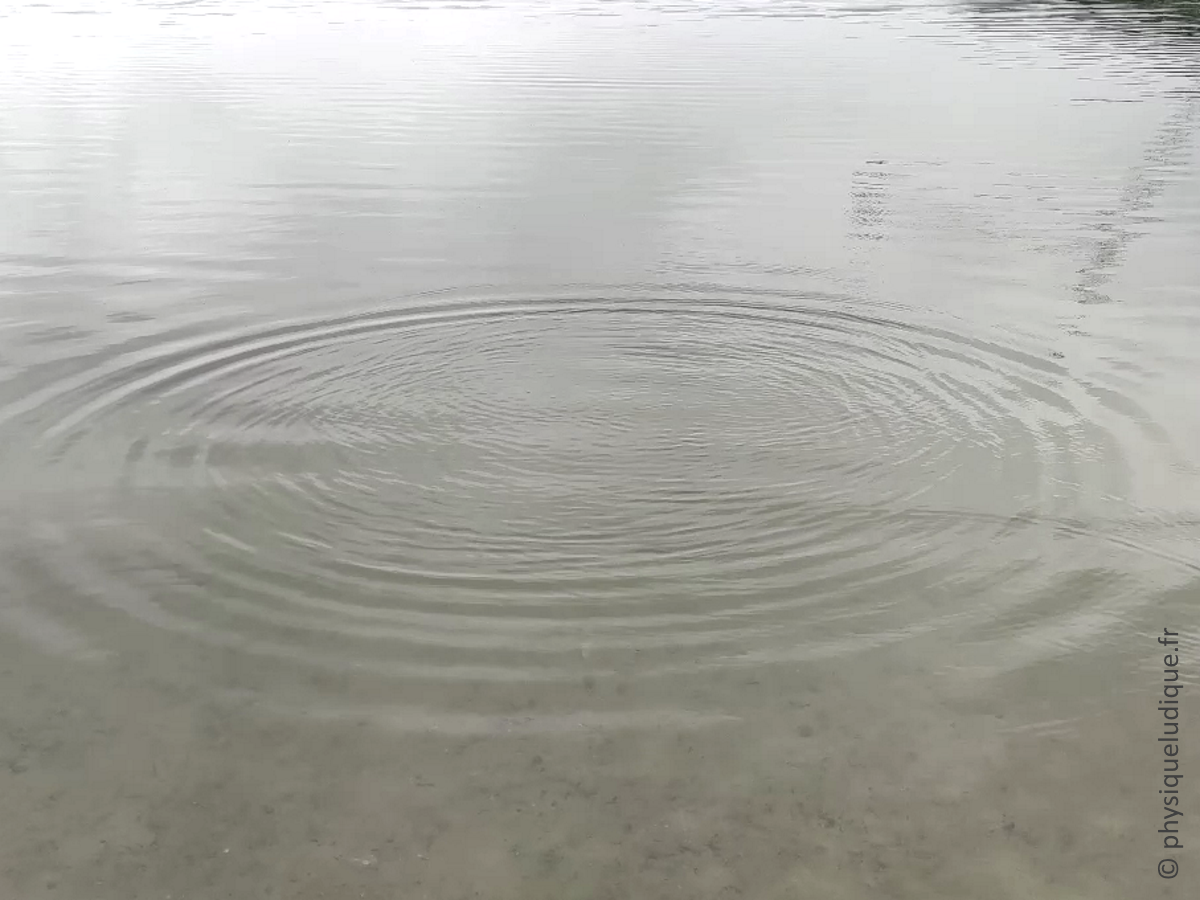
\includegraphics[scale=0.2]{im_intro.png}
    \caption{[1] Image d'une pierre jetée dans une étendue d'eau calme}
    \label{}
\end{figure}

Dans la nature, en particulier dans la mer, on peut observer des comportements particuliers lorsque les vagues rencontrent des fentes, des obstacles ou encore qu'elles se rencontrent entre elles.

\begin{figure}[H]
\centering
\begin{minipage}{0.45\textwidth}
  \centering
  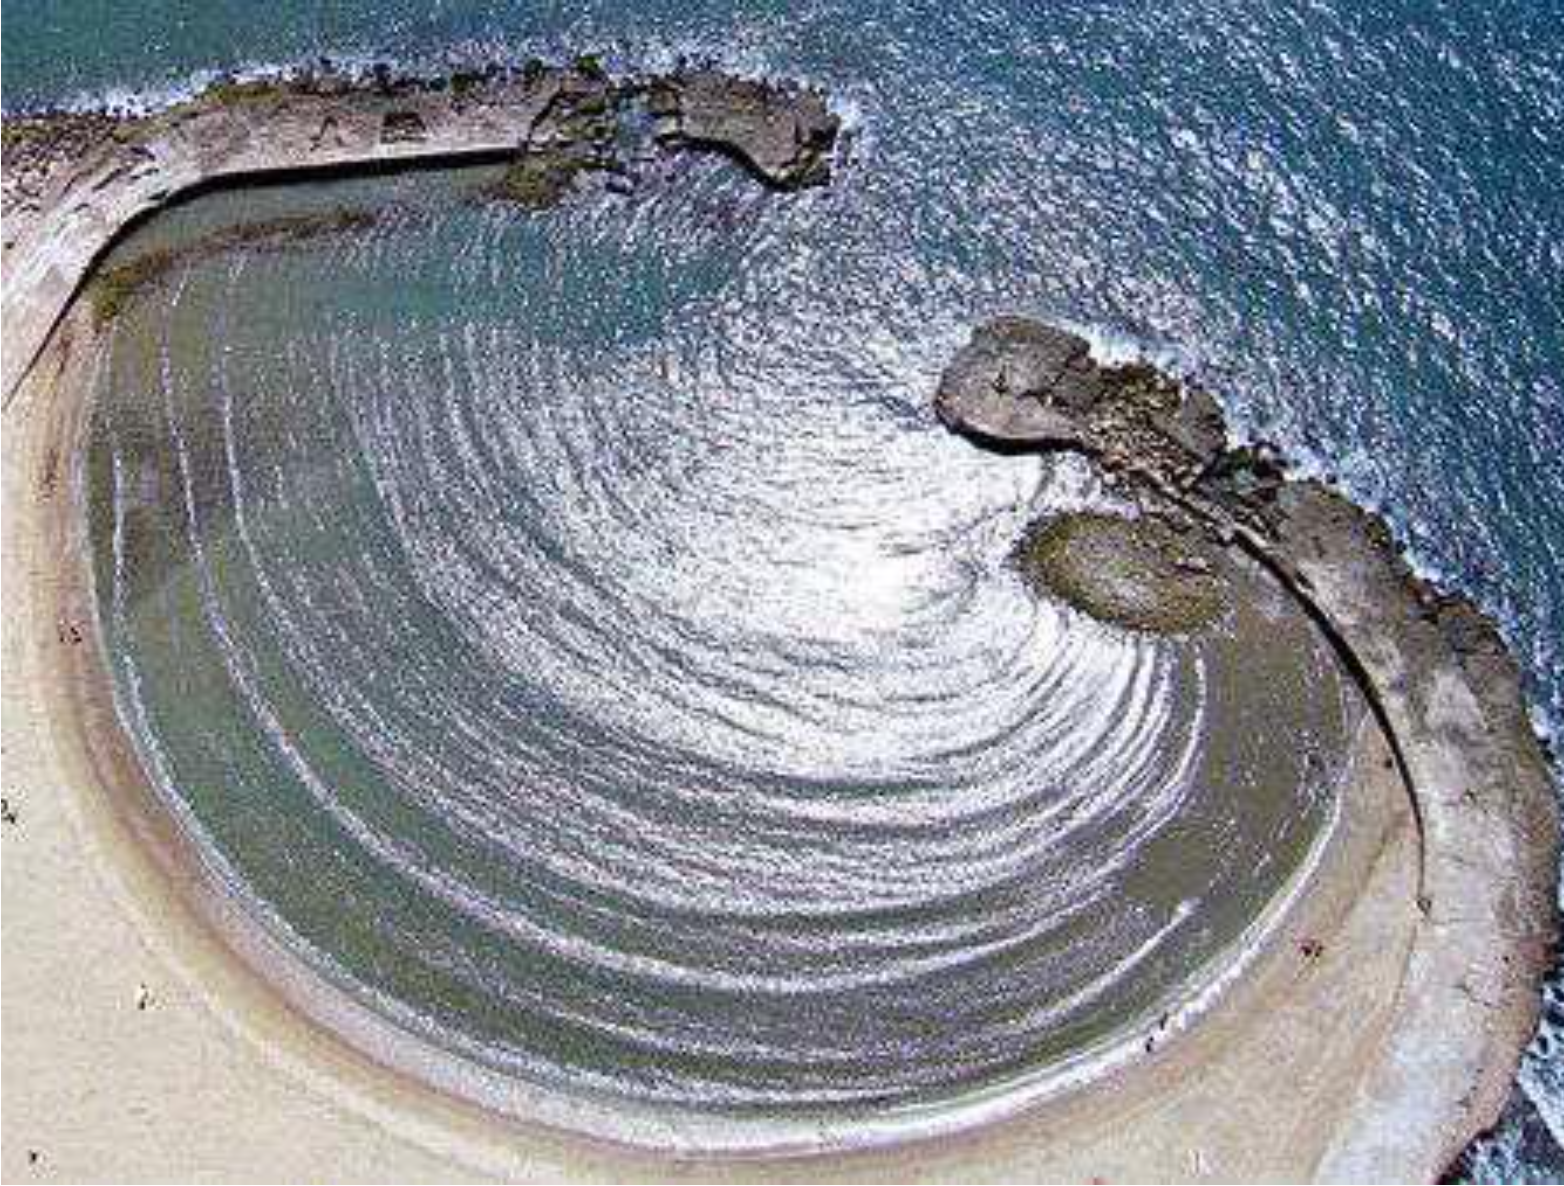
\includegraphics[scale=0.2]{intro_diff.png}
  \caption{[2] Image de la houle dans une plage circulaire}
  \label{fig:s1}
\end{minipage}\hfill
\begin{minipage}{0.45\textwidth}
  \centering
  \includegraphics[scale=0.15]{intro_inter.png}
  \caption{[3] Image de la houle dans le port de Saint-Jean de Luz}
  \label{fig:s2}
\end{minipage}
\end{figure}
%Explication
Lors de ce mini projet de physique expérimentale, nous allons essayer de répondre à ces nombreuses questions en cherchant de manière plus générale à caractériser les ondes à la surface des liquides. En particulier, nous allons regarder si ces ondes de surface obéissent bien à la relation générale de dispersion à la surface des liquides. Nous allons aussi regarder le comportement de ces ondes en présence d'autres ondes ou en présence d'une fente, en étudiant les phénomènes  d'interférences et de diffraction.

\chapter{Montage et principe}

\section{Montage}
\begin{figure}[H]
    \centering
    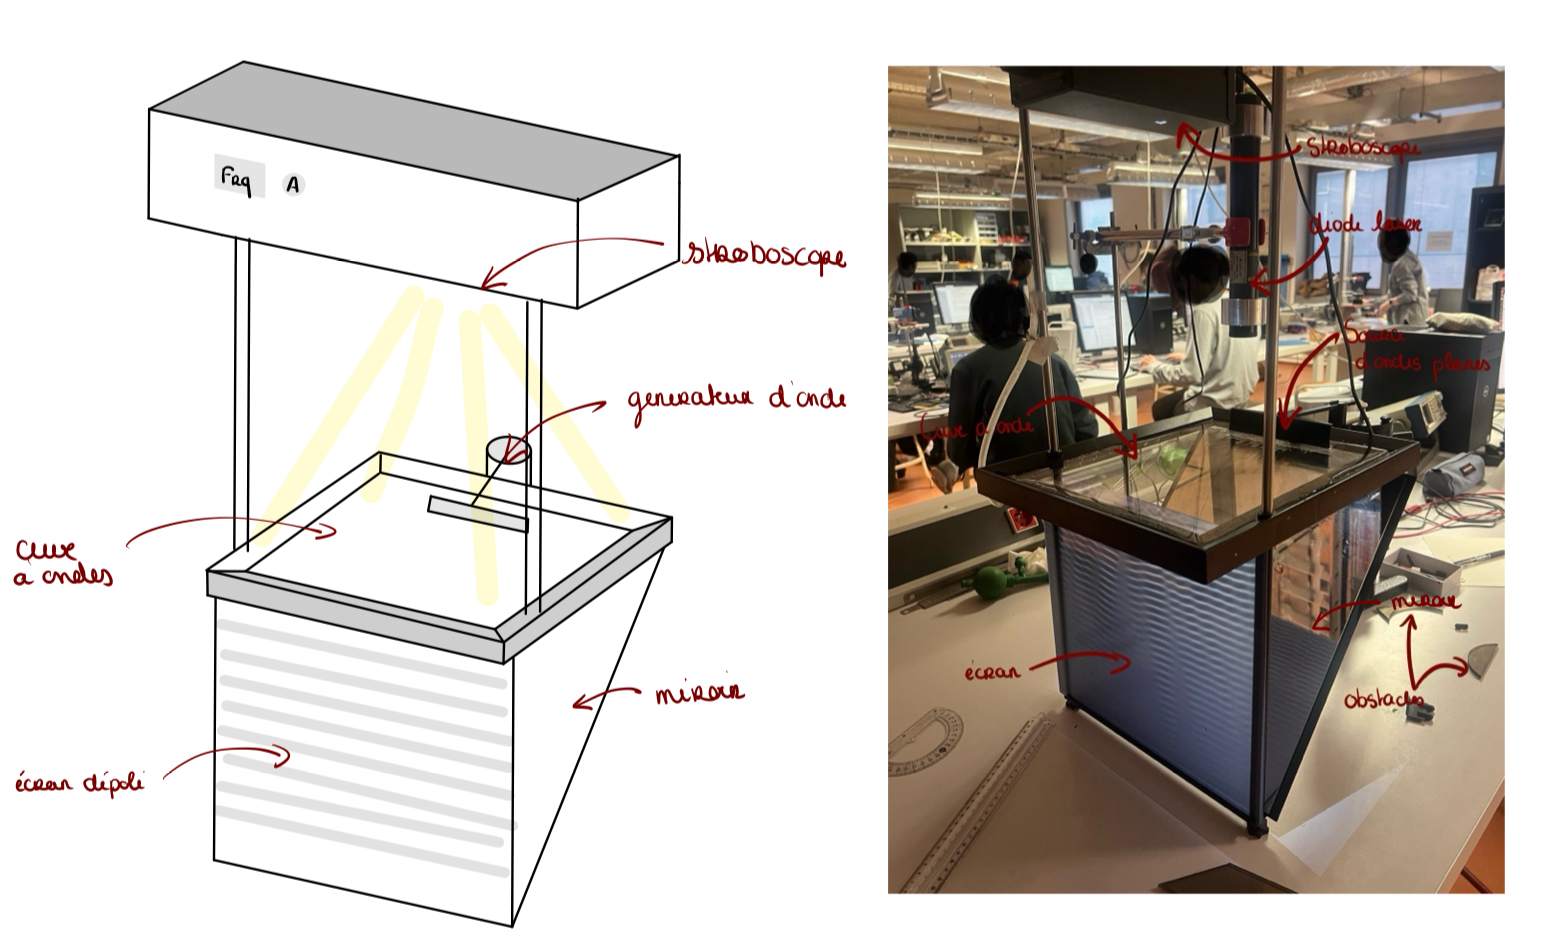
\includegraphics[scale=0.2]{montage.png}
    \caption{Schéma et photo du montage}
    \label{}
\end{figure}
Le montage utilisé pour les expériences est toujours le même. Nous avons à notre disposition une cuve à ondes pour faire nos expériences. Ce montage se compose de plusieurs éléments :
\begin{itemize}[label=\ding{220}]
    \item un générateur d'ondes, qui fait vibrer un accessoire pour générer l'onde. Cet accessoire, en fonction de sa forme, peut générer une onde plane, ou une ou plusieurs ondes circulaires (de même amplitude et de même fréquence).
    \item un bac où on y met un liquide (ici de l'eau distillée ou un mélange avec de l'eau distillée).
    \item un stroboscope qui délivre des flash lumineux périodiques (en fonction de la fréquence des ondes générées) de façon à pouvoir effectuer les mesures plus facilement.
    \item un miroir qui reflète la lumière sur l'écran.
    \item un écran dépoli pour visualiser les ondes générées sur le plan d'eau.
\end{itemize}

Remarque : On observe sur l'écran des zones sombres et des zones claires, on peut donc se poser la question, à quelle zone correspond les maximums ? et les minimums ?\\
Pour répondre à cette question, on peut utiliser le schéma suivant : 

\begin{figure}[H]
    \centering
    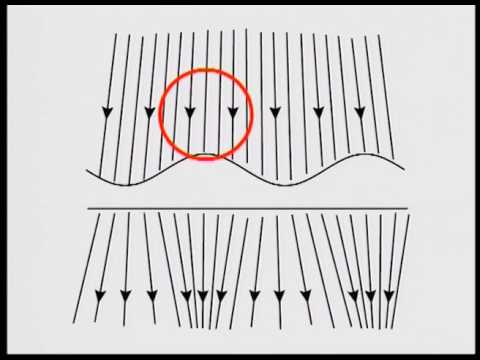
\includegraphics[scale=0.35]{zones.jpg}
    \caption{[4] Comportement des faisceaux lumineux}
    \label{fig:enter-label}
\end{figure}

On voit donc qu'après son passage à la surface de l'eau, la lumière converge lorsqu'elle passe par un maximum (une crête) donc on aura à ces endroits des zones claires, et la lumière diverge lorsqu'elle passe par un minimum (un creux) on aura donc à ces endroits une zone foncée. On peut donc dire que la surface de l'eau se comporte comme un lentille convergente ou divergente en fonction des endroits.

\section{Justification des incertitudes}
Lors des expériences de ce projet nous avons réalisé plusieurs mesures, en particulier des mesures de longueurs d'onde sur l'écran dépoli. Ces mesures ont toutes des incertitudes de type B, dues à l'instrument de mesure et à l'expérimentateur. Nous n'avons pas pris en compte les incertitudes sur les appareils (en particulier les incertitudes sur la fréquence) car n'avons pas trouvé dans la documentation la précision de l'appareil. L'expression de ces incertitudes est donc : $\frac{i}{\sqrt{12}}$ avec $i$ l'intervalle de certitude.

\section{Calcul de l'échelle}

Lors des différentes expériences, on réalise des mesures sur l'écran de la cuve à ondes, il faut donc calculer l'échelle pour pouvoir avoir les valeurs réelles de nos mesures. \\

On utilise un objet qui mesure $14,35 cm$ avec un intervalle de certitude de $0,2 cm$ donc $(14,350 \pm 0,058) cm$ et on réalise une deuxième mesure mais cette fois-ci de l'image de l'objet sur l'écran : $27,00 cm$ avec un intervalle de certitude de $0,7 cm$ donc $(27,00 \pm 0,21) cm$.\\

On trouve donc que l'échelle (rapport entre la mesure réelle et ce qui est mesuré) est de $(0,5315 \pm 0,0085)$.




\chapter{Expériences}
\section{Relation de dispersion}

\subsection{But et procédure}
 On cherche à voir si les ondes à la surface des différents fluides obéissent bien à la relation générale de dispersion des ondes à la surface des liquides (formule issue de la documentation) : $$\omega^2=(gk+\frac{\gamma}{\rho}k^3) \tanh{(hk})$$
 avec $\gamma$ la tension de surface en $N.m^{-1}$, $\omega$ la pulsation en $rad.s^{-1}$, $g = 9,81 m.s^{-2}$ l'accélération de la pesanteur,  $k = \frac{2 \pi}{\lambda}$ le nombre d'onde en $m^{-1}$, $\rho$ la masse volumique en $g.L^{-1}$, et $h$ la hauteur d'eau en $m$.

\begin{itemize}[label=\ding{99}]
    \item On fait des mesures de la longueur d'onde en fonction de la fréquence à une hauteur d'eau fixée (1,15 cm et 1,30 cm) pour de l'eau distillée, puis avec un mélange d'eau et quelques de gouttes de liquide vaisselle, et enfin avec un mélange d'eau et glycérol concentré à 32,4\%.
    \item On trace la pulsation au carré en fonction de $k$, ce qui correspond normalement à la courbe de la relation de dispersion, et on essaye d'en déduire la valeur de la tension de surface pour chaque expérience avec un ajustement non linéaire.
\end{itemize}

\subsection{Mesures et graphes}

Les mesures de longueurs d'onde (en milimètres) trouvées en fonction des fréquences (en Hertz) sont :

\begin{table}[H]
\centering
\caption{Tableau des longueurs d'ondes en mm}
\label{tab:freq}
\scriptsize{\begin{tabular}{c|c|c|c|c|c|c|c|c|c|c|c|c|c|c}
    Frq ($Hz$) : &  $10$ & $15$ & $20$ & $25$ & $30$ & $35$ & $40$ & $45$ & $50$ & $55$ & $60$ & $65$ & $70$ & $75$ \\
    \hline
    Exp 1, $\lambda$ : & $25,25$ & $14,62$ & $9,11$ & $11,16$ & $7,640$ & $6,757$ & $6,07$ & $5,514$ & $5,218$ & $5,005$ & $4,555$ & $4,25$ & $4,052$ & $3,898$ \\
    Exp 1, $u(\lambda$) : & 0,38 & 0,38 & 0,21 & 0,15 & 0,096 & 0,096 & 0,11 & 0,096 & 0,070 & 0,064 &  0,088 & 0,12 & 0,077 & 0,051 \\
    Exp 2, $\lambda$ :  & $22,15$ & $13,73$ & $10,63$ & $8,86$ & $7,59$ & $6,67$ & $5,943$ & $5,527$ & $5,110$ & $4,783$ & $4,418$ & $4,176$ & $3,986$ & $3,720$ \\
    Exp 2, $u(\lambda$) : & 0,51 & 0,26 & 0,12 & 0,18 & 0,15 & 0,12 & 0,070 & 0,077 & 0,059 & 0,055 & 0,048 & 0,055 & 0,043 & 0,045 \\
    Exp 3, $\lambda$ :  & $19,02$ & $11,69$ & $8,86$ & $7,21$ & $6,20$ & $5,39$ & $4,88$ & $4,43$ & $4,19$ & $3,99$ & $3,59$ & $3,45$ & $3,28$ & $3,28$ \\ 
    Exp 3, $u(\lambda$) : & 0,61 & 0,61 & 0,46 & 0,46 & 0,46 & 0,31 & 0,31 & 0,31 & 0,31 & 0,31 & 0,31 & 0,31 & 0,31 & 0,31 \\
    Exp 4, $\lambda$ :  & $19,13$ & $11,87$ & $9,66$ & $7,02$ & $5,98$ & $5,32$ & $4,68$ & $4,38$ & $4,15$ & $3,87$ & $3,19$ & $2,09$ & $2,66$ & $2,02$ \\
    Exp 4, $u(\lambda$) : & 0,92 & 0,92 & 0,77 & 0,77 & 0,77 & 0,61 & 0,61 & 0,46 & 0,46 & 0,46 & 0,46 & 0,46 & 0,31 & 0,31 \\
    Exp 5, $\lambda$ :  & $15,94$ & $11,87$ & $9,67$ & $7,97$ & $6,78$ & $6,20$ & $5,53$ & $5,18$ & $4,78$ & $4,43$ & $4,15$ & $3,89$ & $3,72$ & $3,59$ \\
    Exp 5, $u(\lambda$) : & 1,2 & 0,92 & 0,92 & 0,77 & 0,61 & 0,46 & 0,46 & 0,46 & 0,31 & 0,31 & 0,31 & 0,31 & 0,31 & 0,31 \\
\end{tabular}}
\end{table}
 avec :
\begin{itemize}
     \item \scriptsize{Exp 1 : Eau distillée, $h = 1,15 cm$.}
     \item \scriptsize{Exp 2 : Eau distillée, $h = 1,30 cm$.}
     \item \scriptsize{Exp 3 : Eau distillée + 2 gouttes de liquide vaisselle, $h = 0,725 cm$.}
     \item \scriptsize{Exp 4 : Eau distillée + 15 gouttes de liquide vaisselle, $h = 0,725 cm$.}
     \item \scriptsize{Exp 5 : Eau distillée + Glycérol (concentré à $32\%$), $h = 1,20 cm$.}
 \end{itemize}


\begin{figure}[H]
    \centering
    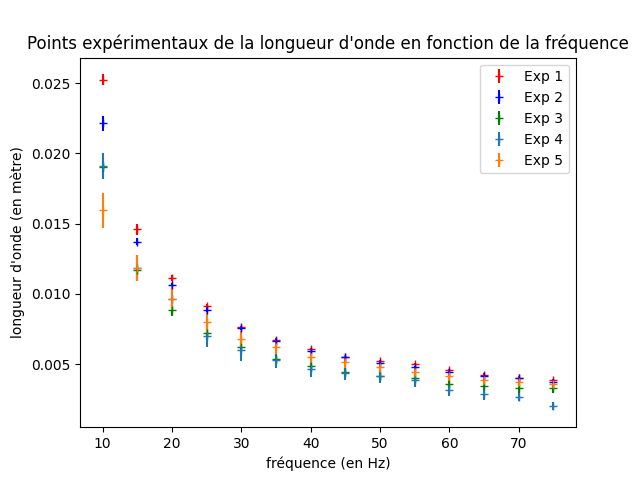
\includegraphics[scale=0.735]{graphe1.png}
    \caption{Graphe des longueurs d'ondes en fonction des fréquences}
    \label{fig:enter-label}
\end{figure}

Les graphes des longueurs d'onde en fonction des fréquences ont tous la même forme; on trace maintenant la pulsation au carré en fonction du nombre d'onde, et on réalise en même temps l'ajustement non linéaire avec la relation de dispersion : $\omega^2=(gk+\frac{\gamma}{\rho}k^3) \tanh{(hk})$ pour trouver le seul paramètre inconnu.\\


\begin{figure}[H]
    \centering
    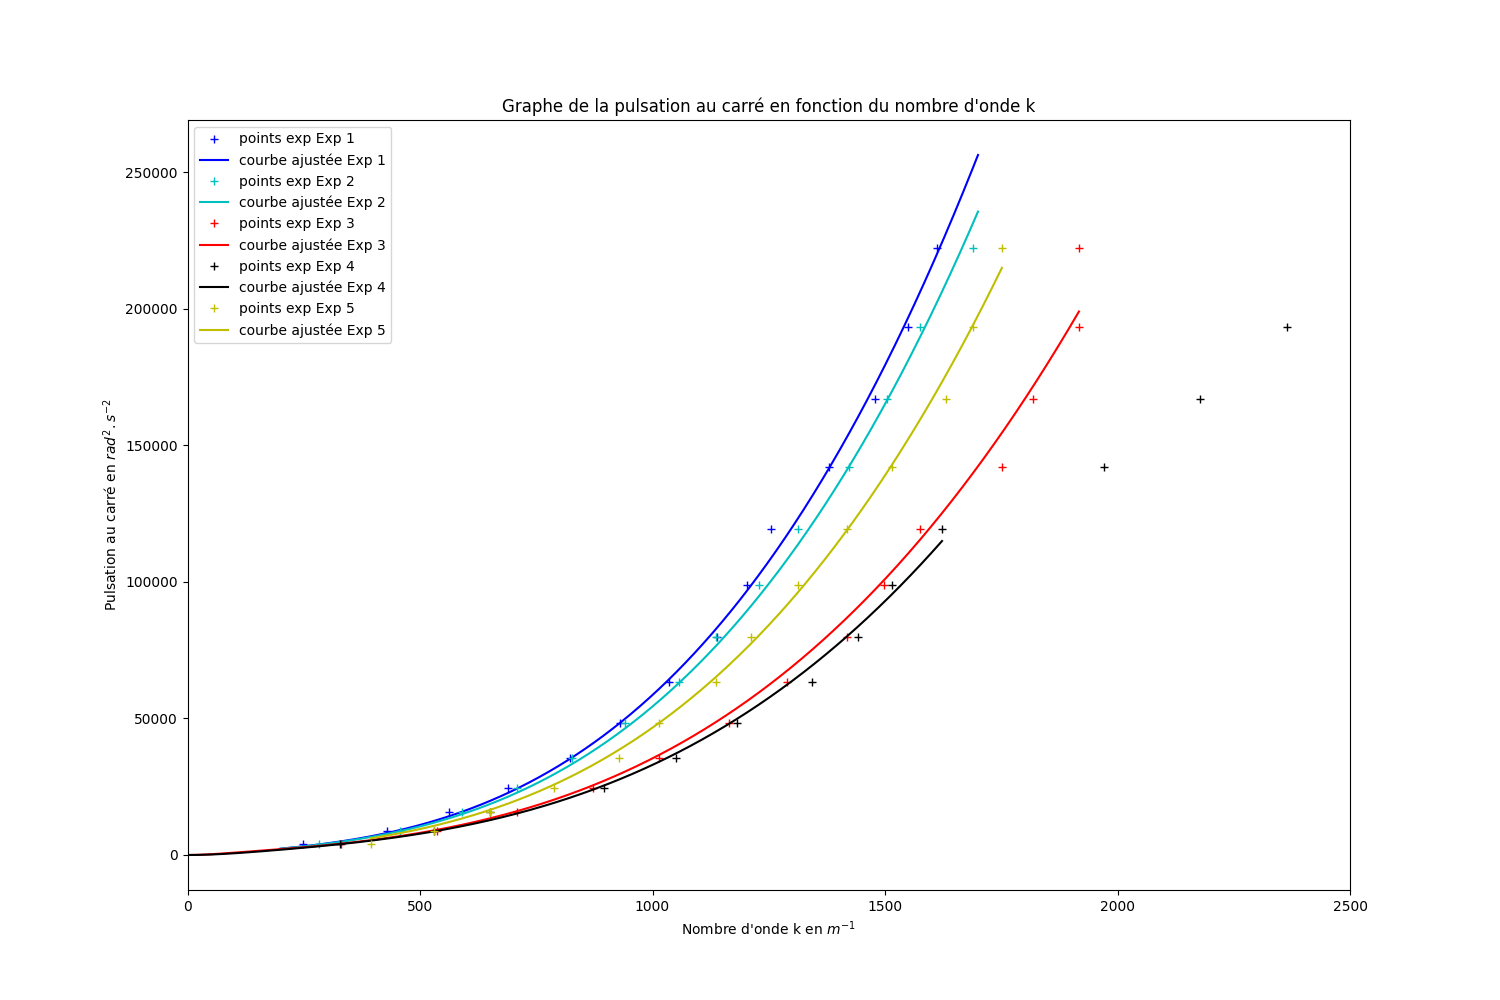
\includegraphics[scale=0.45]{graphe2.png}
    \caption{Graphe de la pulsation au carrée en fonction du nombre d'onde}
    \label{fig:enter-label}
\end{figure}

Remarque : on a préféré mettre tous les résultats trouvés sur le même graphe pour pouvoir les comparer entre eux bien que les graphes soient donc un peu moins compréhensibles.


En effet, les paramètres connus pour les expériences sont $h$ la hauteur d'eau et $\rho$ la masse volumique, et le paramètre inconnu est $\gamma$ la tension de surface :
\begin{itemize}[label=\ding{229}]
    \item Exp 1 : $h = 1,15 cm$, $\rho = 1 000 g.L^{-1}$ et le résultat de l'ajustement donne  $\gamma =  (48,76 \pm 0,48) mN.m^{-1}$
    \item Exp 2 : $h = 1,30 cm$, $\rho = 1 000 g.L^{-1}$ et le résultat de l'ajustement donne  $\gamma = (44,54 \pm 0,42) mN.m^{-1}$
    \item Exp 3 : $h = 0,725 cm$, $\rho = 1 000 g.L^{-1}$ et le résultat de l'ajustement donne  $\gamma = (25,57 \pm 0,56) mN.m^{-1}$
    \item Exp 4 : $h = 0,725 cm$, $\rho = 1 000 g.L^{-1}$ et le résultat de l'ajustement donne $\gamma = (23,16 \pm 0,46) mN.m^{-1}$
    \item Exp 5 : $h = 1,20 cm$, $\rho = 1 084 g.L^{-1}$ et le résultat de l'ajustement donne$\gamma = (39, 91 \pm 0, 48) mN.m^{-1}$
\end{itemize}

Remarque : pour l'Exp 4 (eau distillée avec 15 gouttes de liquide vaisselle), le résultat de l'ajustement nous donnait une valeur absurde avec une incertitude très grande, on a donc refait cet ajustement en se limitant au 10 premières valeurs. En effet, on peut l'expliquer parce qu'à partir d'un certain moment (fréquences hautes), on a vu l'apparition de bulles, ce qui a probablement faussé nos mesures.

\subsection{Ondes capillaires ou gravitationnelles?}
La documentation du projet nous explique que de manière générale, les ondes à la surface d’un liquide peuvent se classer en deux catégories. Celles-ci dépendent de leur longueur d’onde, et donc de ce qui est à l’origine de leur force de rappel (la force qui tend à ramener le liquide vers son état d’équilibre, c’est-à-dire de surface lisse) : 

\begin{itemize}[label=\ding{105}]
    \item les ondes de gravité (pour des longueurs d’onde supérieures à 1 cm), dont la force de rappel est dûe principalement à la gravité; c’est le cas des vagues sur l’océan par exemple. Dans ce cas, le terme dominant dans la relation de dispersion est  $gk$.
    \item les ondes capillaires (pour des longueurs d’onde de l’ordre du millimètre), dont la force de rappel est dûe principalement à la tension de surface $\gamma$. Dans ce cas, le terme dominant dans la relation de dispersion est $\frac{\gamma}{\rho}k^3$
    %\item les ondes capillaires (pour des longueurs d’onde inférieures à 1 millimètre), dont la force de rappel est dûe principalement à la tension de surface $\gamma$. Dans ce cas, le terme dominant dans la relation de dispersion est $\frac{\gamma}{\rho}k^3$
\end{itemize}

Les longueurs d'ondes mesurées lors de nos expériences varient entre 30 mm et 2 mm. Donc d'après ce qui est expliqué ci-dessus, on ne peut pas clairement dire s'il s'agit plutôt d'ondes de surface ou d'ondes capillaires. Néanmoins, on a mis en évidence le fait que la tenison de surface a une influence sur les longueurs d'onde, donc on peut quand même supposer que ces ondes sont plutôt capillaires. De plus, si on reprend par exemple notre première expérience (eau distillée, $h=1,15 cm$) et qu’on trace les fonctions $\omega^2=\frac{\gamma}{\rho}k^3 \tanh{(hk)}$ et $\omega^2=gk\tanh{(hk)}$ avec $\gamma = 49 mN.m^{-1}$ par dessus, on obtient le graphe suivant:

% Les longueurs d'ondes mesurées lors de nos expériences sont entre 30 mm et 2 mm. Donc d'apres ce qui est dit ci-dessus, on ne peut pas clairement dire si ce sont plutot des ondes de surface ou des ndes capillaires. Néanmoins, on a mis en evidence le fait le que tenison de surface avait un influnec sur les longueurs d'onde, on peut donc quand même supposer que ce sont des ondes plutôt capillaires. Pour en être sur, prenons les valeurs trouvée à la première experience ($h = 1,15 cm$ avec de l'au distillée uniquement), et traçon la courbe de la relation de dispersion avec uniquement le terme domimant pour le ondes capillaures, et séparemement, le courbe avec uniquement le terme domimant pour le ondes gravitationnelles :

\begin{figure}[H]
    \centering
    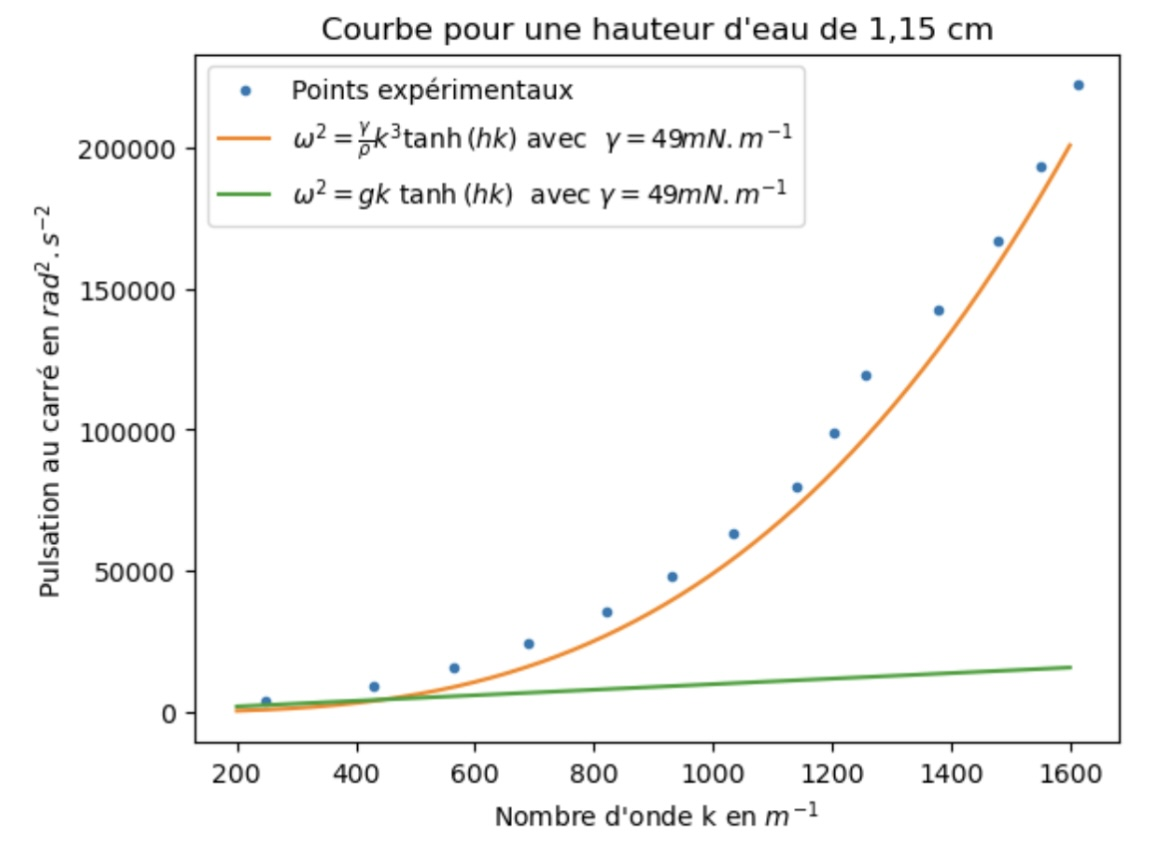
\includegraphics[scale=0.8]{graphe6.jpeg}
    \caption{Courbe des composantes de la relation de dispersion pour des ondes gravitationnelle et capillaire}
    \label{fig:enter-label}
\end{figure}

%mettre un nouveau graphe avec en plus le terme domimant pour le ondes gravitationnelles.


On observe que les points expérimentaux se rapprochent plus de la courbe de la relation de dispersion avec uniquement le terme dominant $\frac{\gamma}{\rho}k^3$. On peut donc conclure, comme nous avons pu le supposer précédemment, que les ondes observées lors de ces expériences peuvent être essentiellement caractérisées comme capillaires. 

% On voit ici que les points expériemnetaux se rapporchent plus de la courbe de la relation de dispersion avec uniquement le terme dominant pour les ondes capillaires. On peut donc dire, comme nous avon spu les supposer plus tôt, que les ondes observées lors de ces expériences se rapprochent plus des ondes capillaires.


\subsection{Vitesse de phase}
On peut aussi se demander à quelle vitesse l’onde se propage, c’est-à-dire s’intéresser à sa vitesse de phase $v_{\phi}$. On trouve dans la documentation qu’elle obéit à la formule  $v_{\phi} = \lambda f$. En reprenant les longueurs d’ondes associées à leur fréquence et les longueurs d'ondes obtenues dans la première expérience, on peut calculer la vitesse de phase de l’onde dans l’eau distillée pour chaque fréquence:

\begin{table}[H]
\centering
\caption{Tableau des viteses de phase en $cm.s^{-1}$}
\label{tab:vphi}
\scriptsize{\begin{tabular}{c|c|c|c|c|c|c|c|c|c|c|c|c|c|c}
    Frq ($Hz$) : &  $10$ & $15$ & $20$ & $25$ & $30$ & $35$ & $40$ & $45$ & $50$ & $55$ & $60$ & $65$ & $70$ & $75$ \\
    \hline
    Exp 1, $\lambda$ (mm) : & $25,25$ & $14,62$ & $9,11$ & $11,16$ & $7,640$ & $6,757$ & $6,07$ & $5,514$ & $5,218$ & $5,005$ & $4,555$ & $4,25$ & $4,052$ & $3,898$ \\
    Exp 1, $u(\lambda$) (mm) : & 0,38 & 0,38 & 0,21 & 0,15 & 0,096 & 0,096 & 0,11 & 0,096 & 0,070 & 0,064 &  0,088 & 0,12 & 0,077 & 0,051 \\
    \hline
    Exp 1, $v_{\phi}$ :  & 25,25 & 21,92 & 22,32 & 22,78 & 22,92 & 23,65 & 24,30 & 24,81 & 26,09 & 27,53 & 27,33 & 27,64 & 28,37 & 29,23 \\
    Exp 1, $u(v_{\phi}$) : & 0,38 & 0,58 & 0,43 & 0,38 & 0,29 & 0,34 & 0,44 & 0,43 & 0,35 & 0,35 & 0,53 & 0,80 & 0,5 & 0,38 \\
\end{tabular}}
\end{table}

%\begin{figure}[H]
    %\centering
    %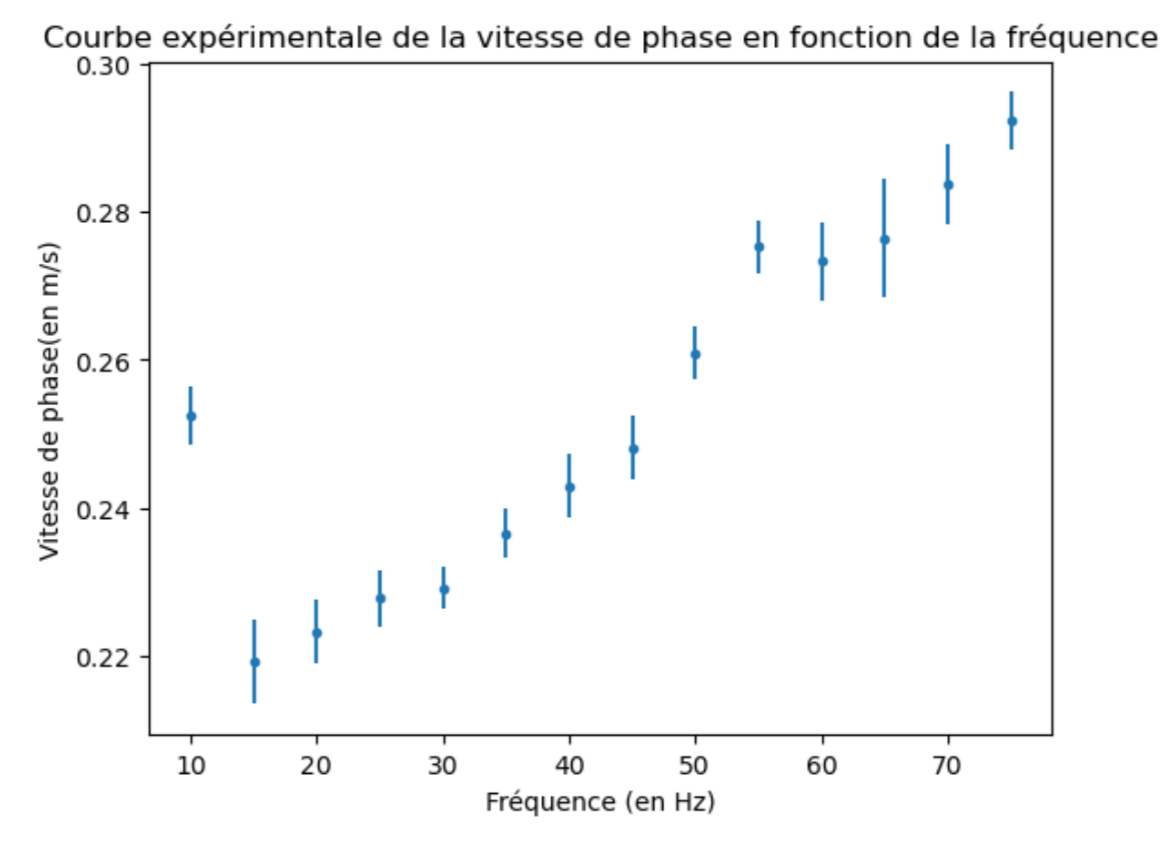
\includegraphics[scale=0.27]{graphe4.jpeg}
    %\caption{Courbe expérimentale de la vitesse de phase en fonction de la fréquence}
    %\label{fig:enter-label}
%\end{figure}

Cela nous permet de conclure que dans l’eau distillée, l’onde se propage à une vitesse allant de 0,2 à 0,3 $m.s^{-1}$, et que celle-ci augmente lorsque la fréquence imposée augmente. 

\subsection{Interprétation des résultats obtenus et conclusion}
\begin{itemize}[label = \ding{217}]
    \item On voit sur les graphes que les valeurs correspondent bien au modèle décrit par la relation de dispersion, comme on avait pu le supposer, quel que soit le liquide utilisé.
    \item Lors de ces expériences, nous n'avons pu observer que des ondes capillaires (à cause des contraintes matérielles).
    \item On voit aussi que la hauteur d'eau n'a pas beaucoup d'influence sur les valeurs de longueur d'onde.
    \item Concernant les résultats des ajustements, nous avons fait une première hypothèse, qu'il y ait un problème de mesures pour l'expérience avec le glycérol : 
    \begin{enumerate}
        \item les deux premiers ajustements nous donnaient une valeur de tension de surface de l'eau qui serait entre $44 mN.m^{-1}$ et $49 mN.m^{-1}$,
        \item les deux ajustements suivants nous ont montré que les gouttes de liquide vaisselle faisaient baisser la tension de surface entre $23 mN.m^{-1}$ et $26 mN.m^{-1}$.
        \item par contre pour le dernier ajustement avec le glycérol, nous avons trouvé dans la documentation que la tension de surface de ce dernier devait être de $64mN.m^{-1}$ ce qui n'est pas cohérent avec le résultat trouvé par notre ajustement qui aurait dû être entre $44 mN.m^{-1}$ et $64 mN.m^{-1}$, et qui nous donne $40 mN.m^{-1}$.
     \end{enumerate}
    On en a donc déduit une deuxième hypothèse qui rendrait les résultats plus cohérents entre eux, qu'il y ait un problème d'échelle :
    \begin{enumerate}
        \item la tension de surface de l'eau distillée ne serait pas la bonne : celle trouvée avec les deux premiers ajustements est entre $44 mN.m^{-1}$ et $49 mN.m^{-1}$ alors que dans la documentation on trouve une tension de surface de $70 mN.m^{-1}$.
        \item le résultat des deux ajustements avec le liquide vaisselle, serait toujours cohérent avec le fait que le liquide vaisselle fasse baisser la tension de surface
        \item pour le glycérol, on trouverait par contre un résultat cohérent : si l'eau a une tension de surface de $70 mN.m^{-1}$ et que le glycérol a une tension de surface un peu plus faible, de $64 mN.m^{-1}$, l'ajout du glycérol ferait légèremement baisser la tension de surface, ce qui est le cas car avec l'ajout du glycérol, le tension de surface passe d'entre $44 mN.m^{-1}$ et $49 mN.m^{-1}$, à $40 mN.m^{-1}$.
    \end{enumerate} 
\end{itemize}

On peut conclure de ces expériences que les ondes à la surface des fluides obéissent bien à la relation de dipersion quel que soit le liquide ou le mélange utilisé.

\section{Interférences}


\subsection{But et procédure}
On observe le comportement des fronts d'ondes (ici circulaires) lorsqu'il y a plusieurs sources d'onde et on essaie de l'interpréter.

On utilise une ou plusieurs sources d'ondes, qui génèrent des ondes circulaires, on fait varier la fréquence (en ayant toujours des sources de fréquences identiques) et la distance entre ces deux sources, tout en fixant la hauteur d'eau : 

\begin{itemize}[label=\ding{229}]
    \item 1 source - fréquences : $12, 18, 24, 47 Hz$
    \item 2 sources espacées de $(3,40 \pm 0,23) cm$ - fréquences : $12, 18, 24, 34, 47, 55 Hz$
    \item 2 sources espacées de $(14,10 \pm 0,40) cm$ - fréquences : $12, 18, 24, 34, 47, 55 Hz$
    \item 2 sources espacées de $(8,05 \pm 0,43) cm$ - fréquences : $12, 18, 24, 34, 47, 55 Hz$
    \item 3 sources espacées chacune de $(7,10 \pm 0,40) cm$ - fréquences : $12, 18, 24, 34, 47, 55 Hz$
    \item 3 sources espacées chacune de $(4,05 \pm 0,38) cm$ - fréquences : $12, 18, 24, 34, 47, 55 Hz$
    \item 4 sources espacées chacune de $(4,25 \pm 0,43) cm$ - fréquences : $12, 18, 24, 34, 47, 55 Hz$
\end{itemize}

\subsection{Photos de l'expérience}

Pour chacune des situations on prend une photo et on analyse ensuite ces photos :

\begin{figure}[H]
\centering
\begin{minipage}{0.4\textwidth}
  \centering
  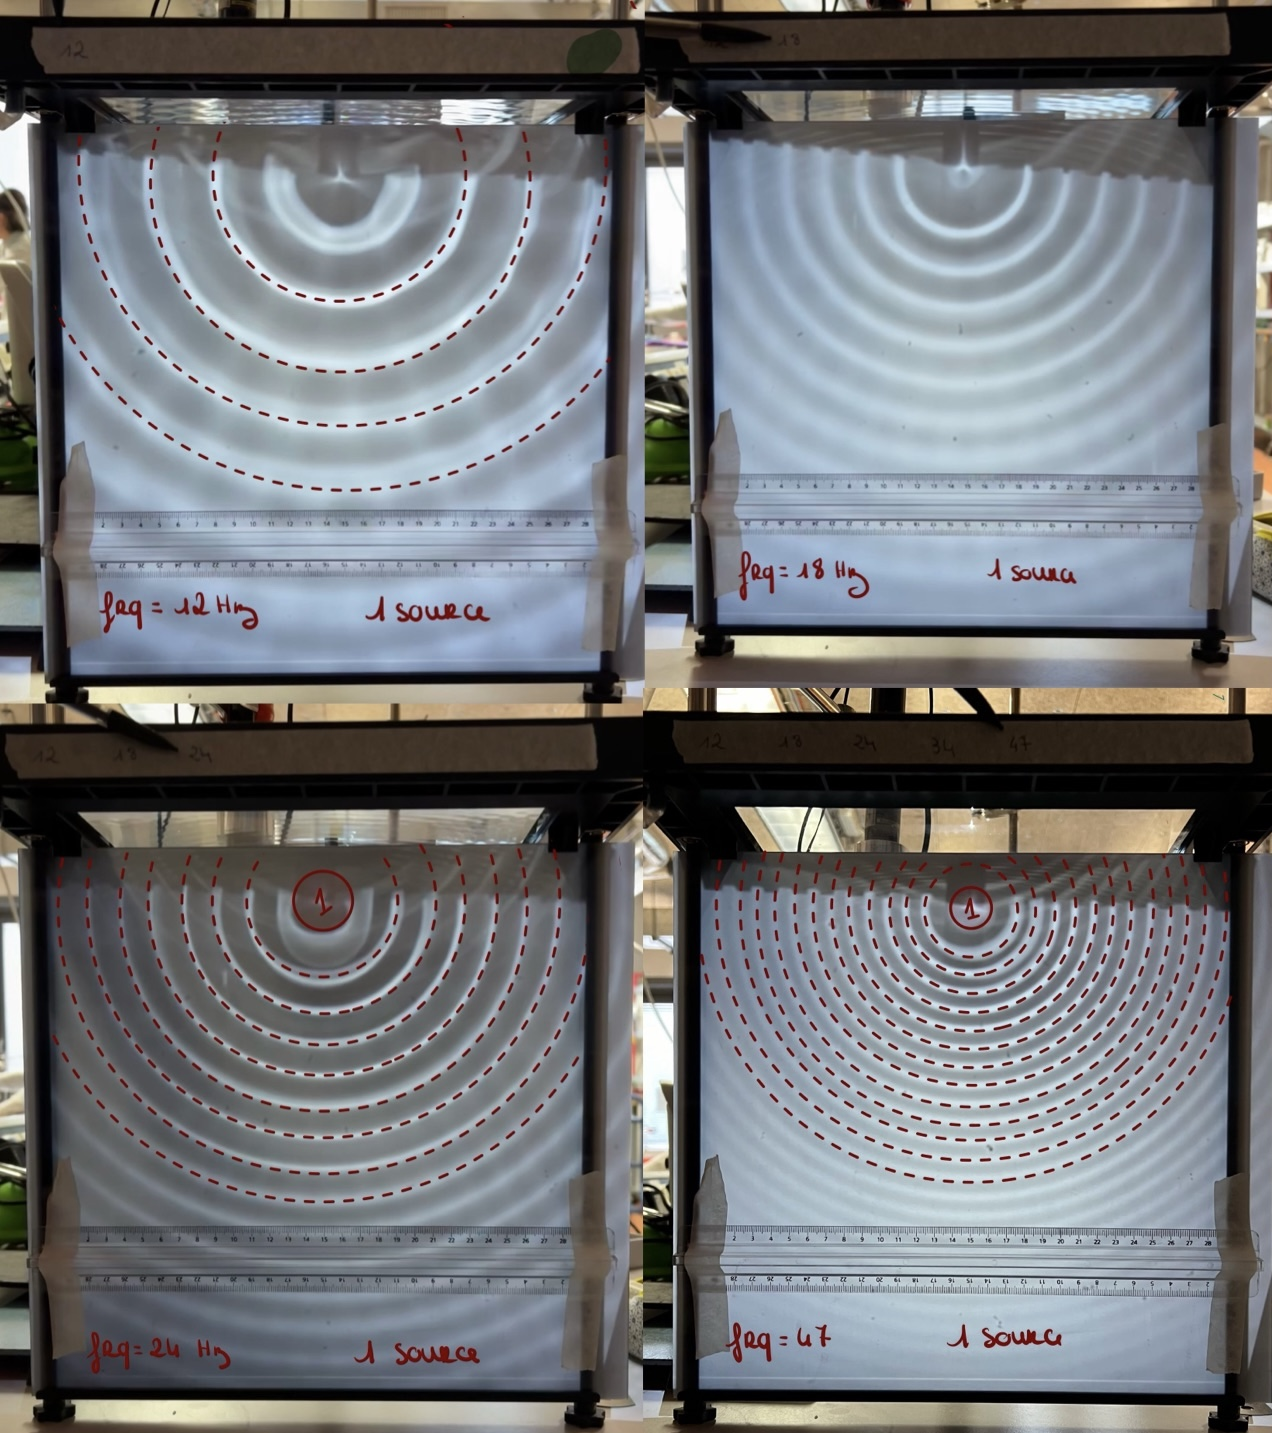
\includegraphics[scale=0.14]{S1.jpg}
  \caption{Photos avec 1 source d'onde}
  \label{fig:s1}
\end{minipage}\hfill
\begin{minipage}{0.5\textwidth}
  \centering
  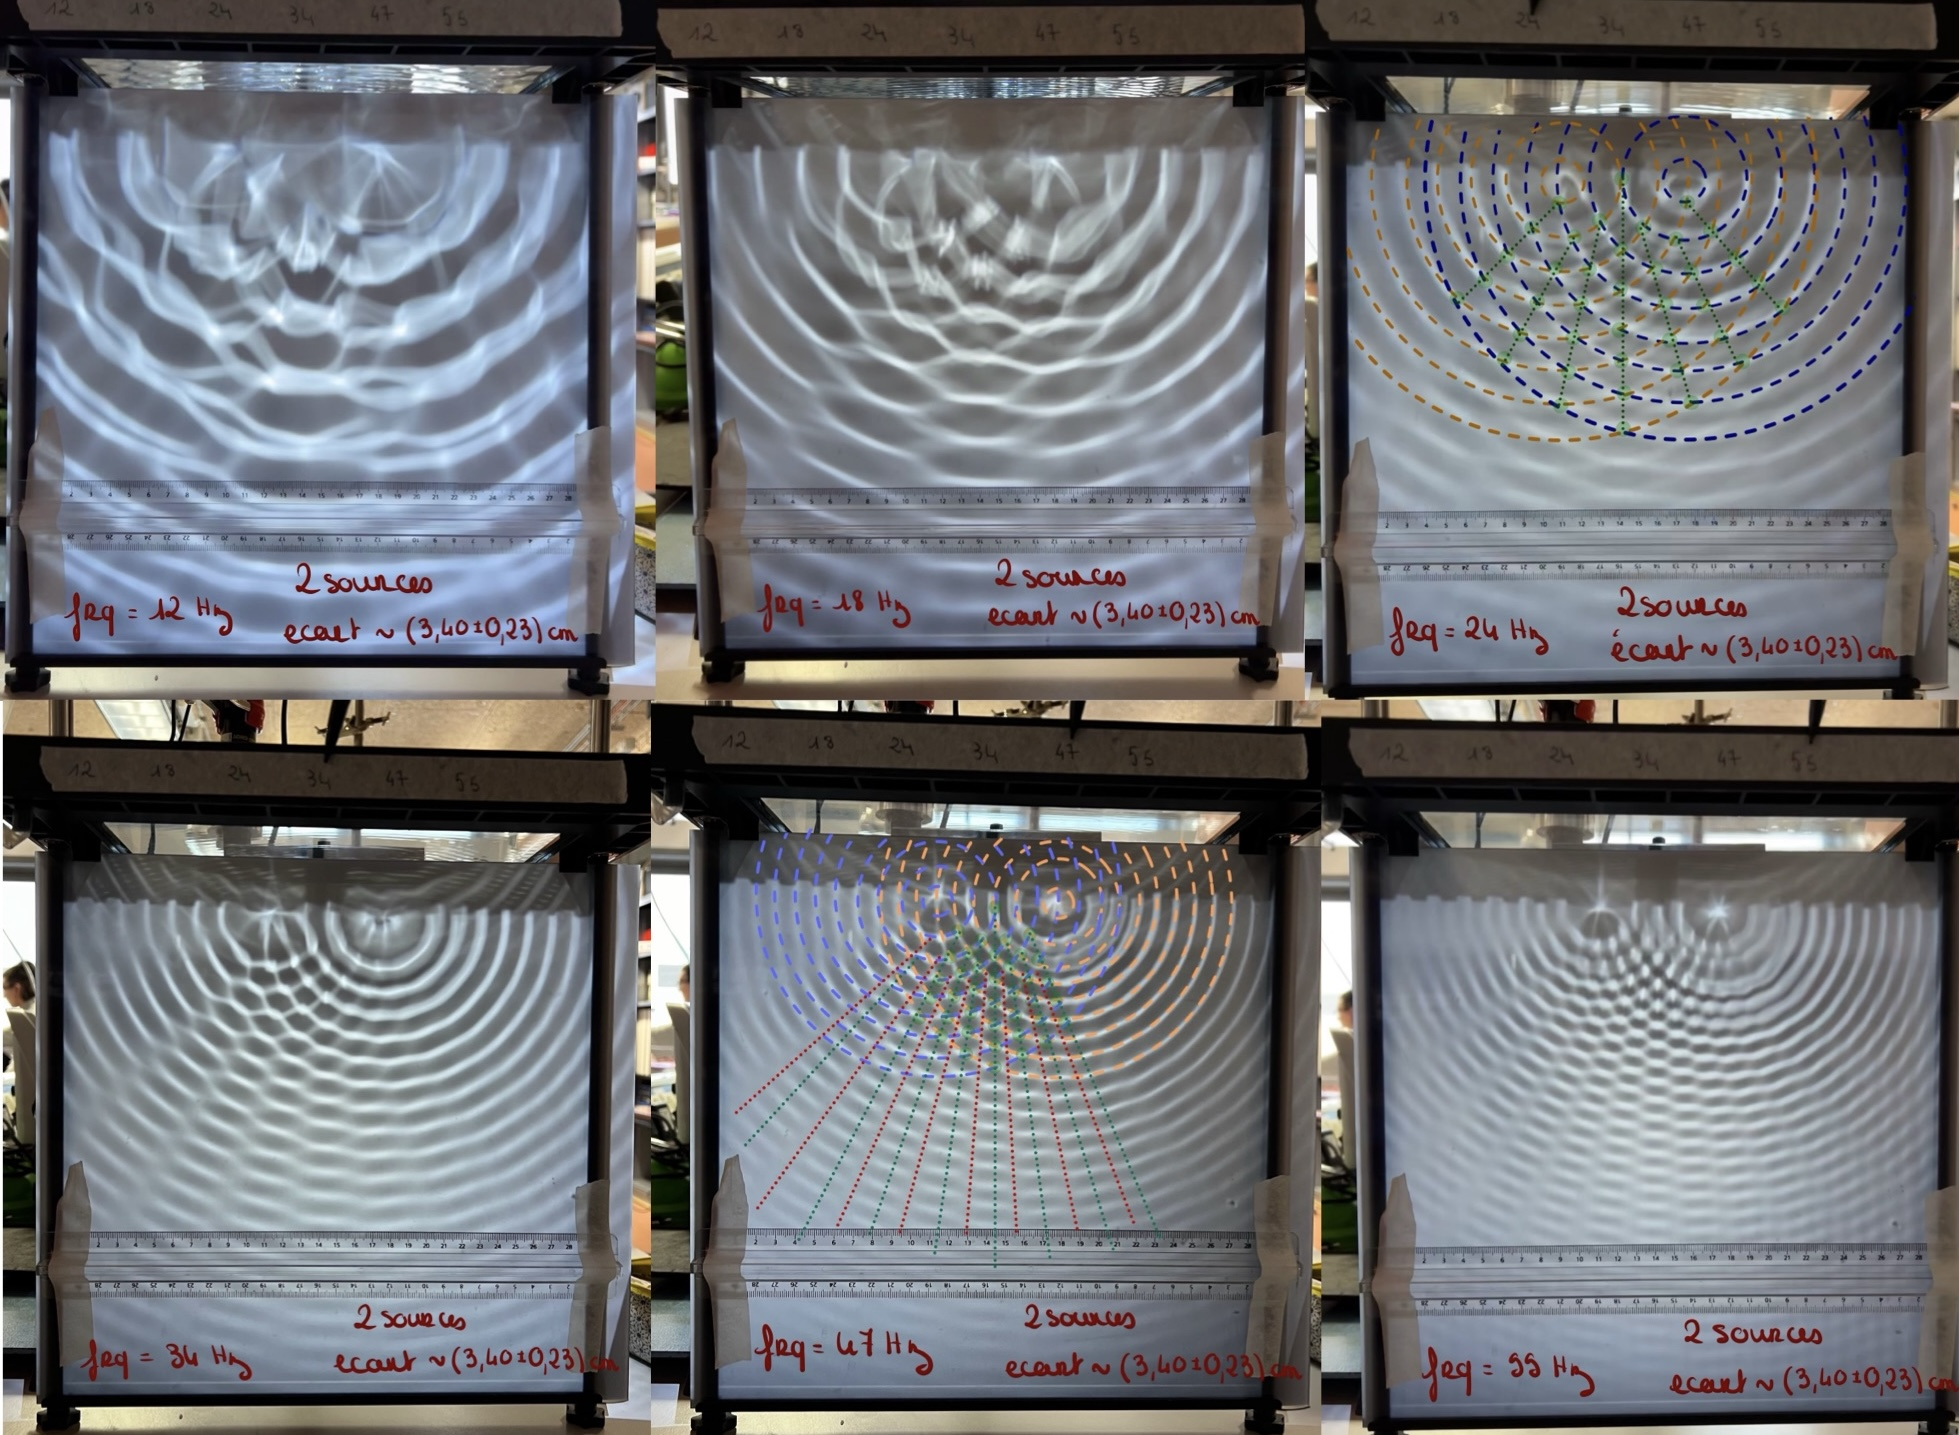
\includegraphics[scale=0.14]{S2P.jpg}
  \caption{Photos avec 2 sources d'onde espacées de 3,40 cm}
  \label{fig:s2}
\end{minipage}
\end{figure}

\begin{figure}[H]
\centering
\begin{minipage}{0.45\textwidth}
  \centering
  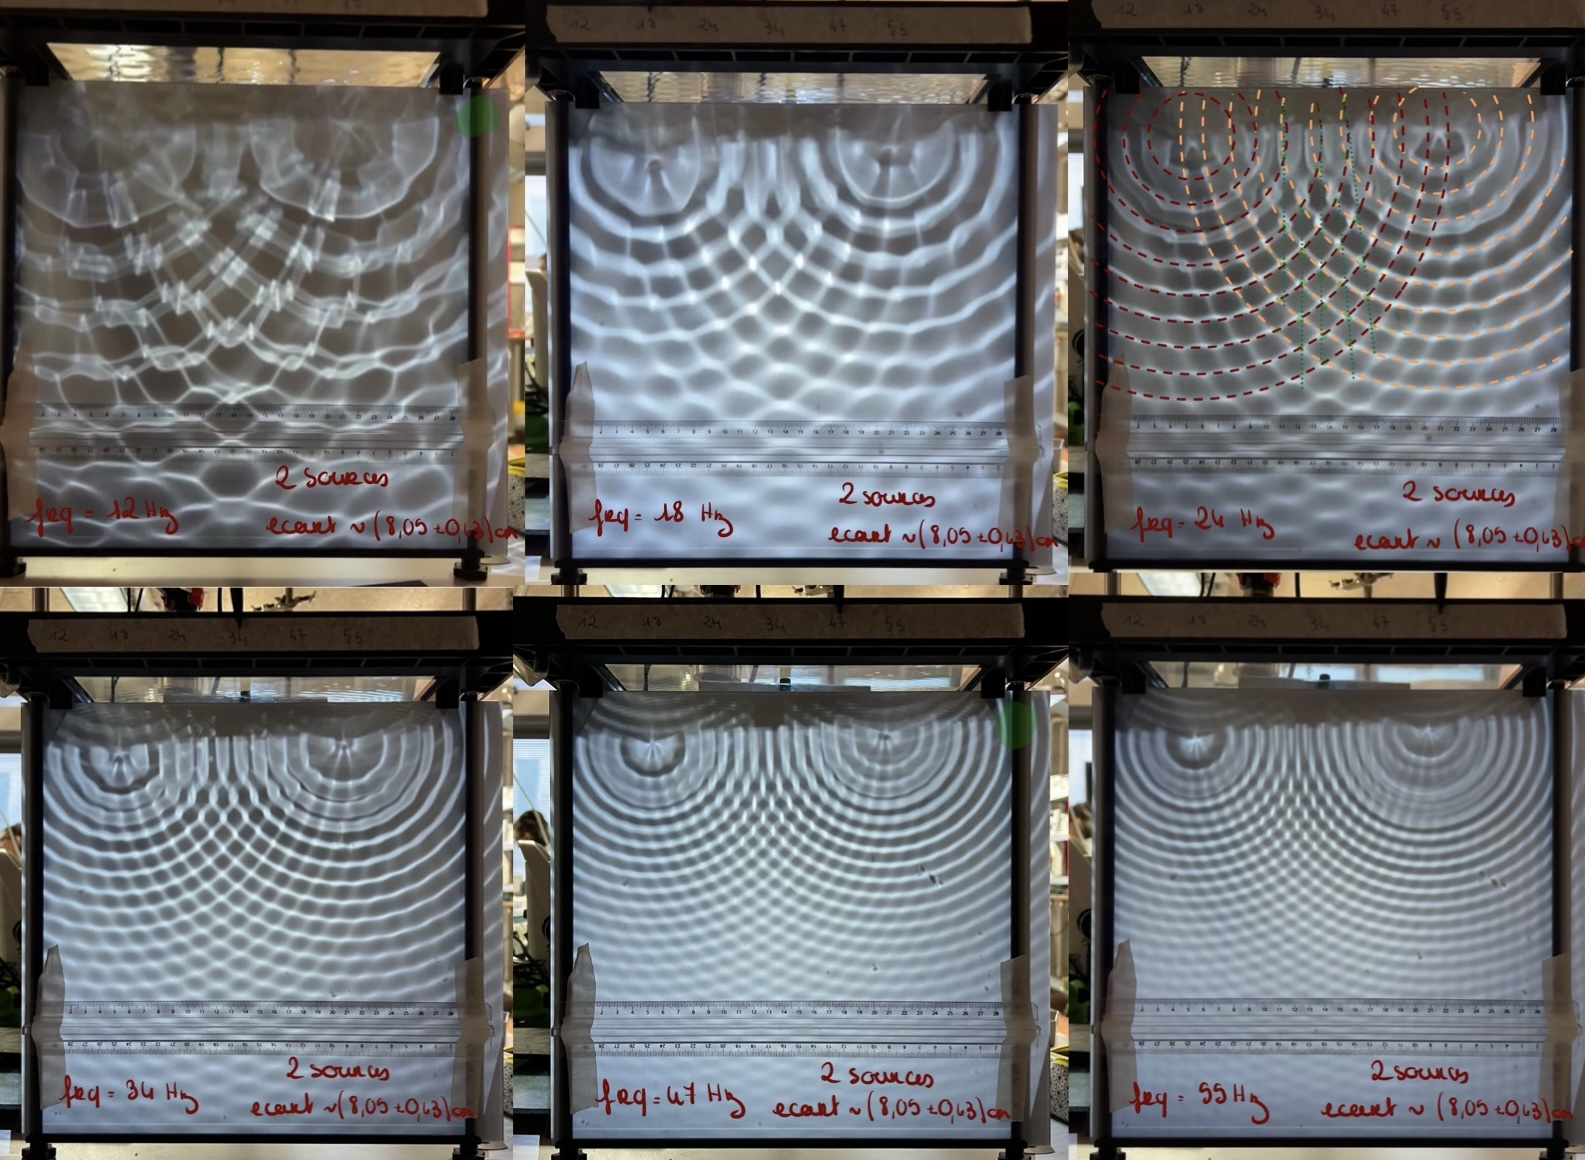
\includegraphics[scale=0.14]{S2M.jpg}
  \caption{Photos avec 2 sources d'onde espacées de 8,05 cm}
  \label{fig:s1}
\end{minipage}\hfill
\begin{minipage}{0.45\textwidth}
  \centering
  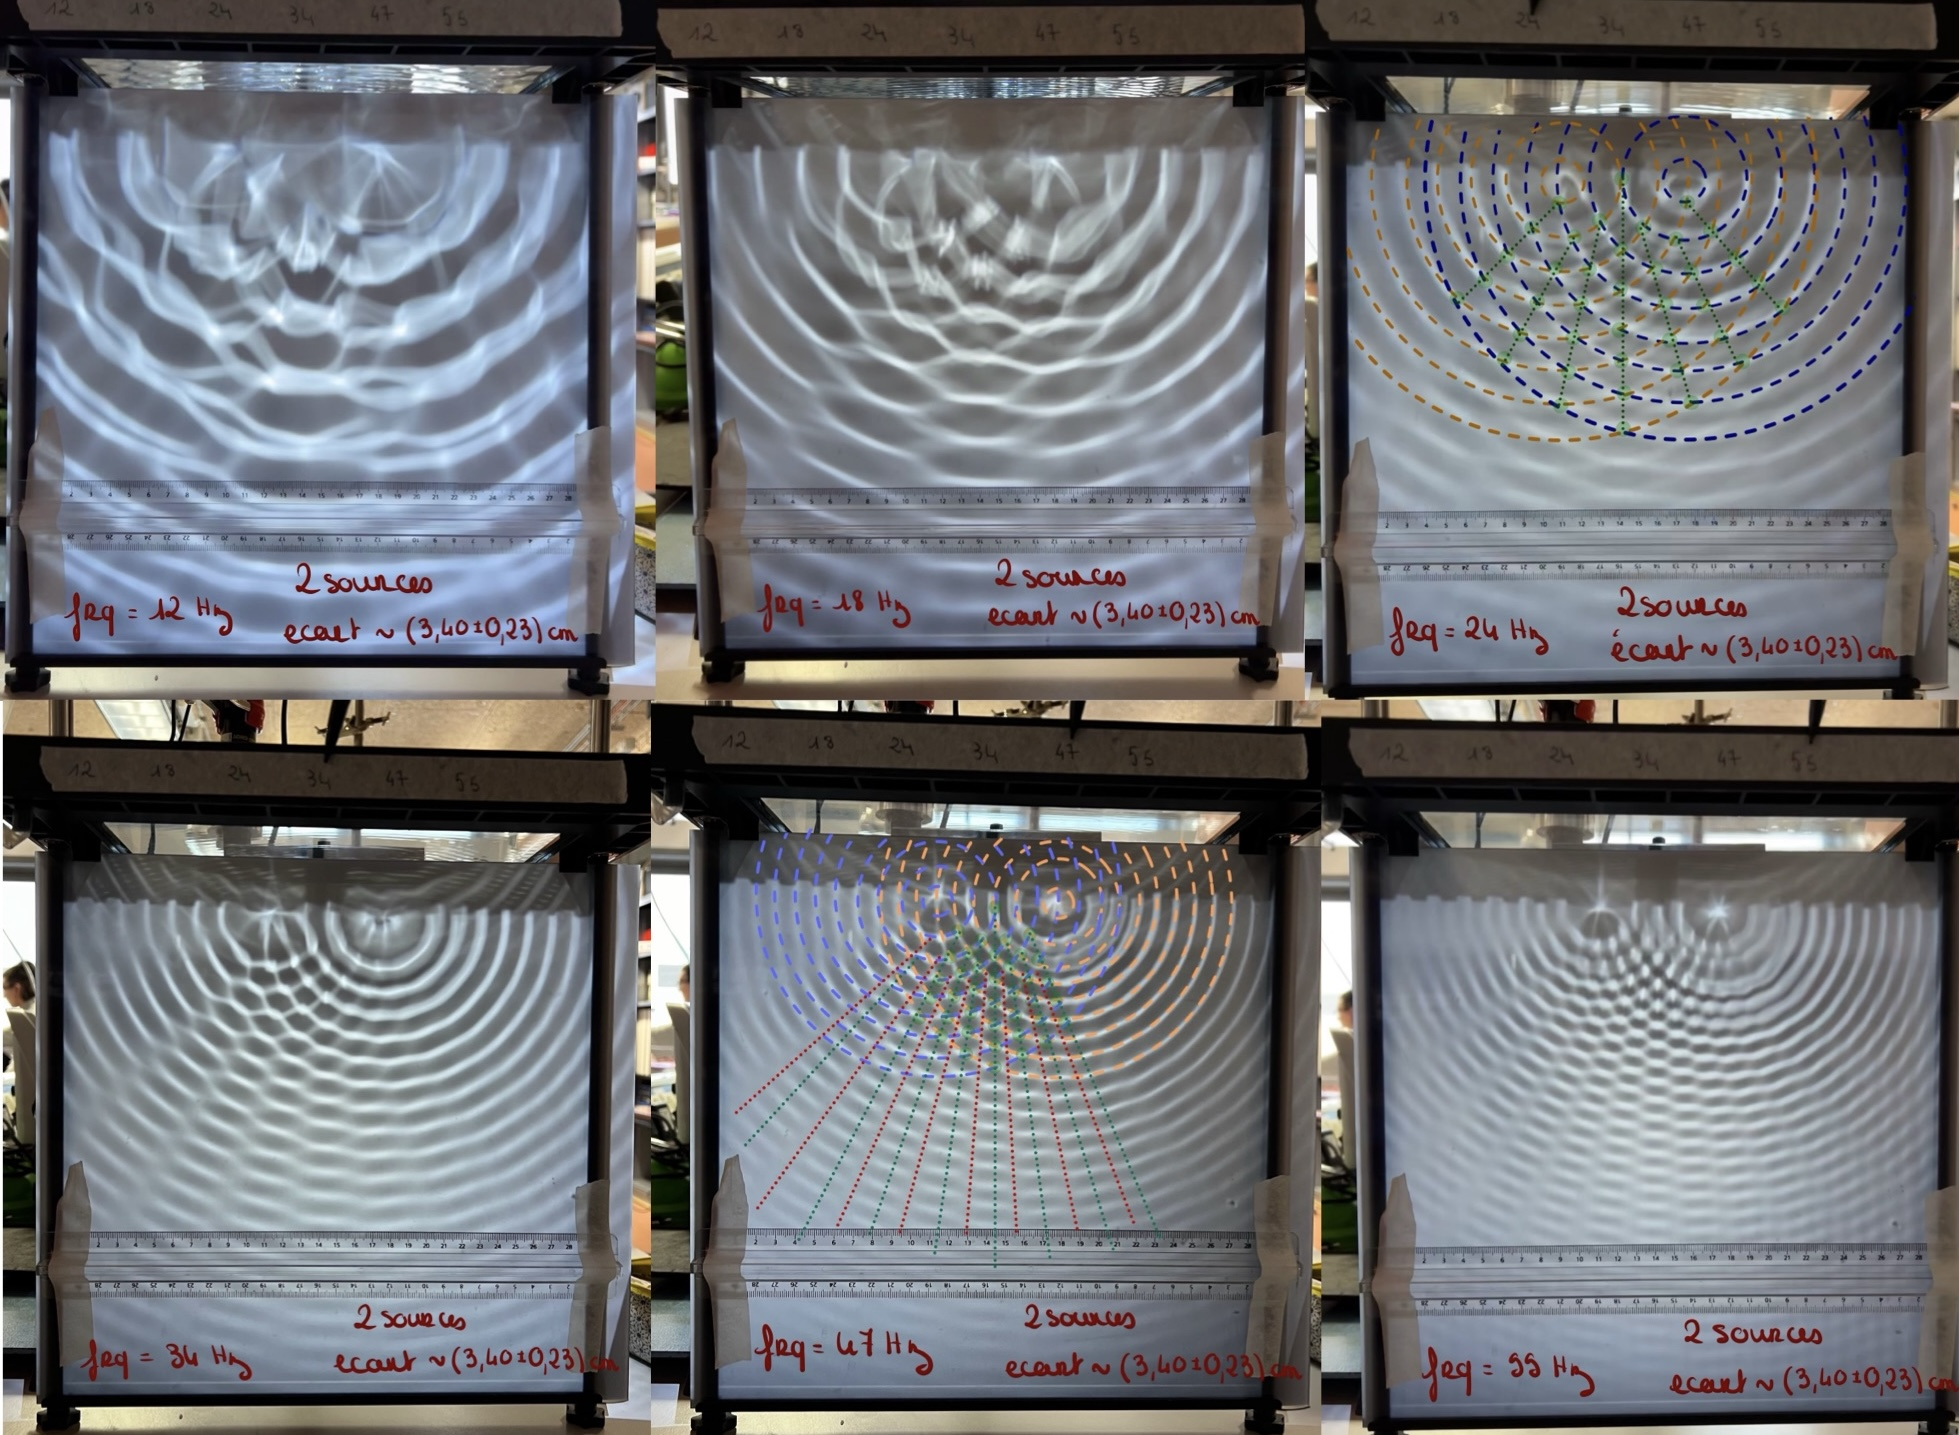
\includegraphics[scale=0.12]{S2P.jpg}
  \caption{Photos avec 2 sources d'onde espacées de 14,10 cm}
  \label{fig:s2}
\end{minipage}
\end{figure}

\begin{figure}[H]
\centering
\begin{minipage}{0.45\textwidth}
  \centering
  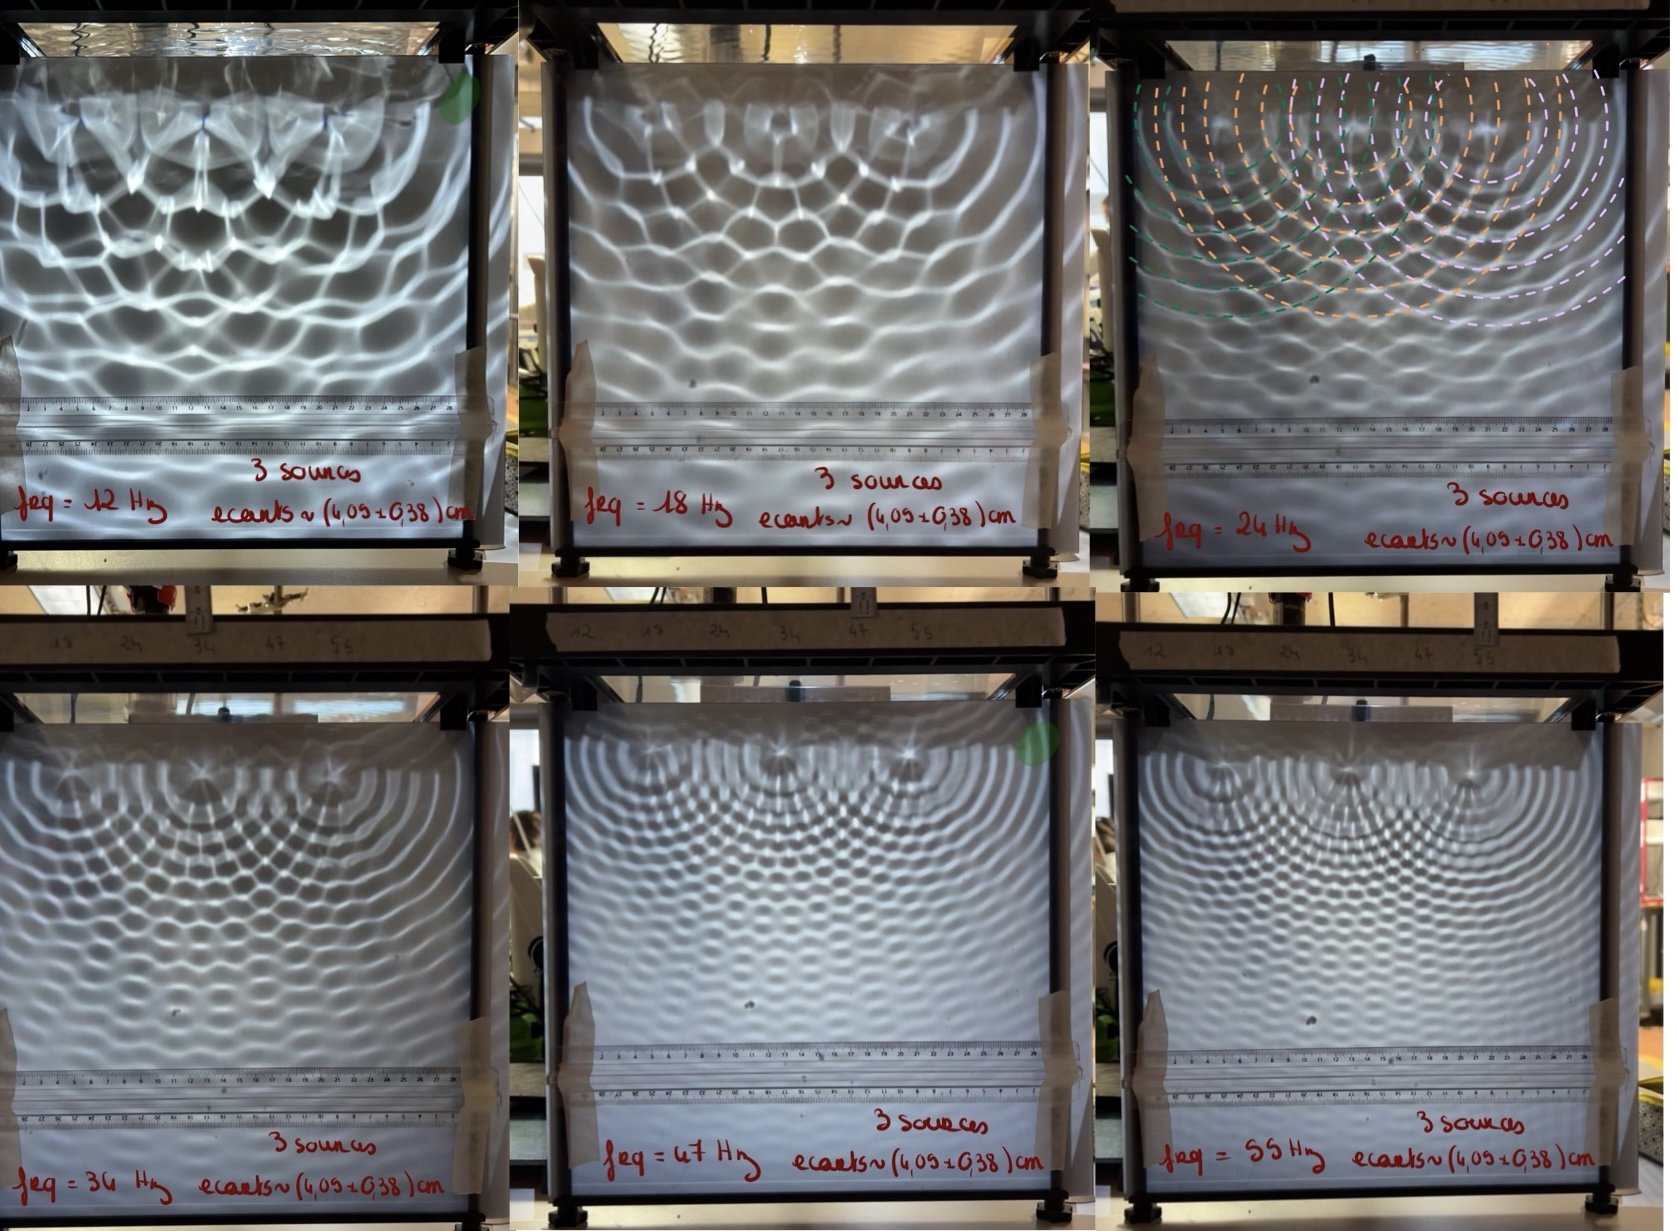
\includegraphics[scale=0.14]{S3P.jpg}
  \caption{Photos avec 3 sources d'onde espacées de 4,04 cm}
  \label{fig:s1}
\end{minipage}\hfill
\begin{minipage}{0.45\textwidth}
  \centering
  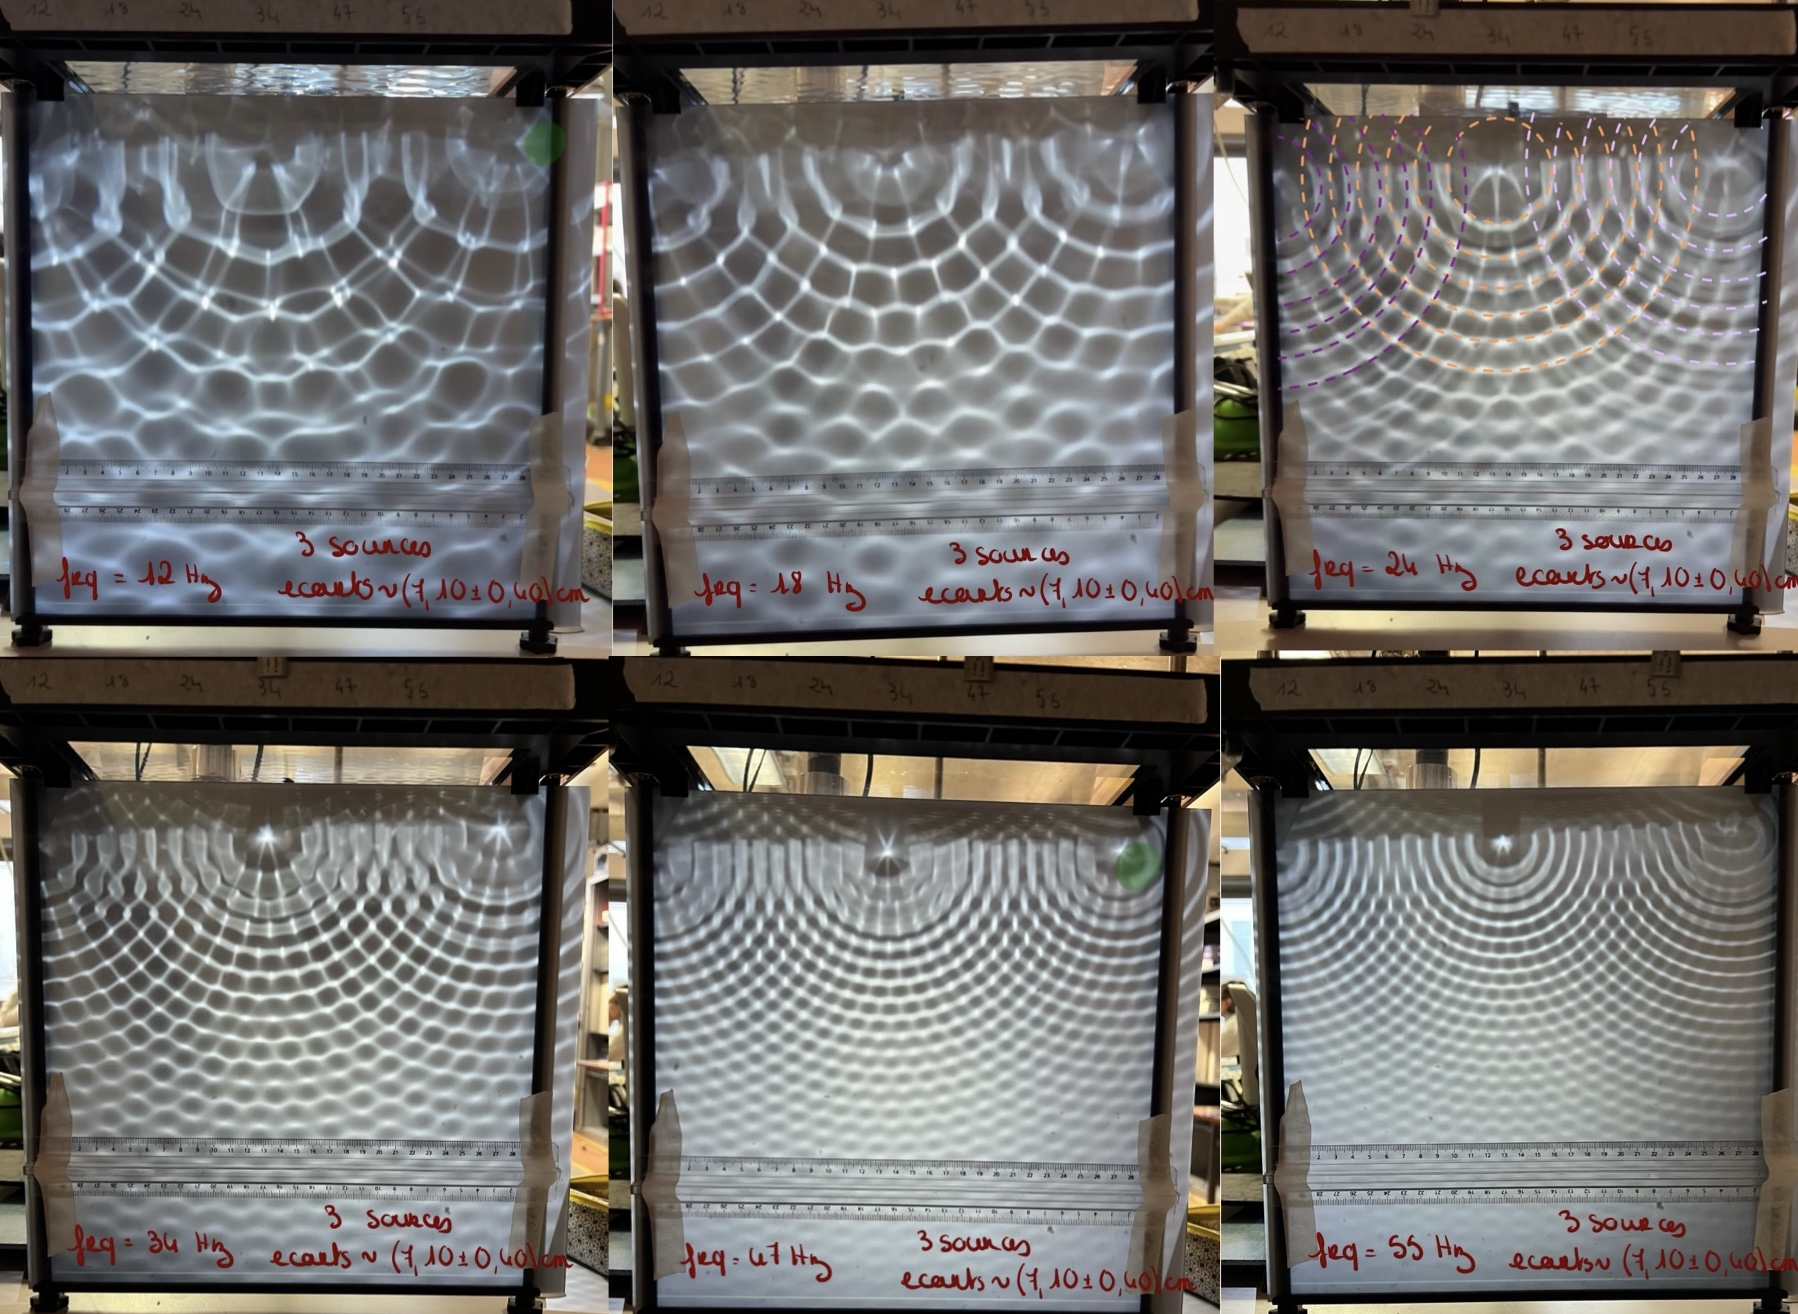
\includegraphics[scale=0.14]{S3M.jpg}
  \caption{Photos avec 3 sources d'onde espacées de 7,10 cm}
  \label{fig:s2}
\end{minipage}
\end{figure}

\begin{figure}[H]
    \centering
    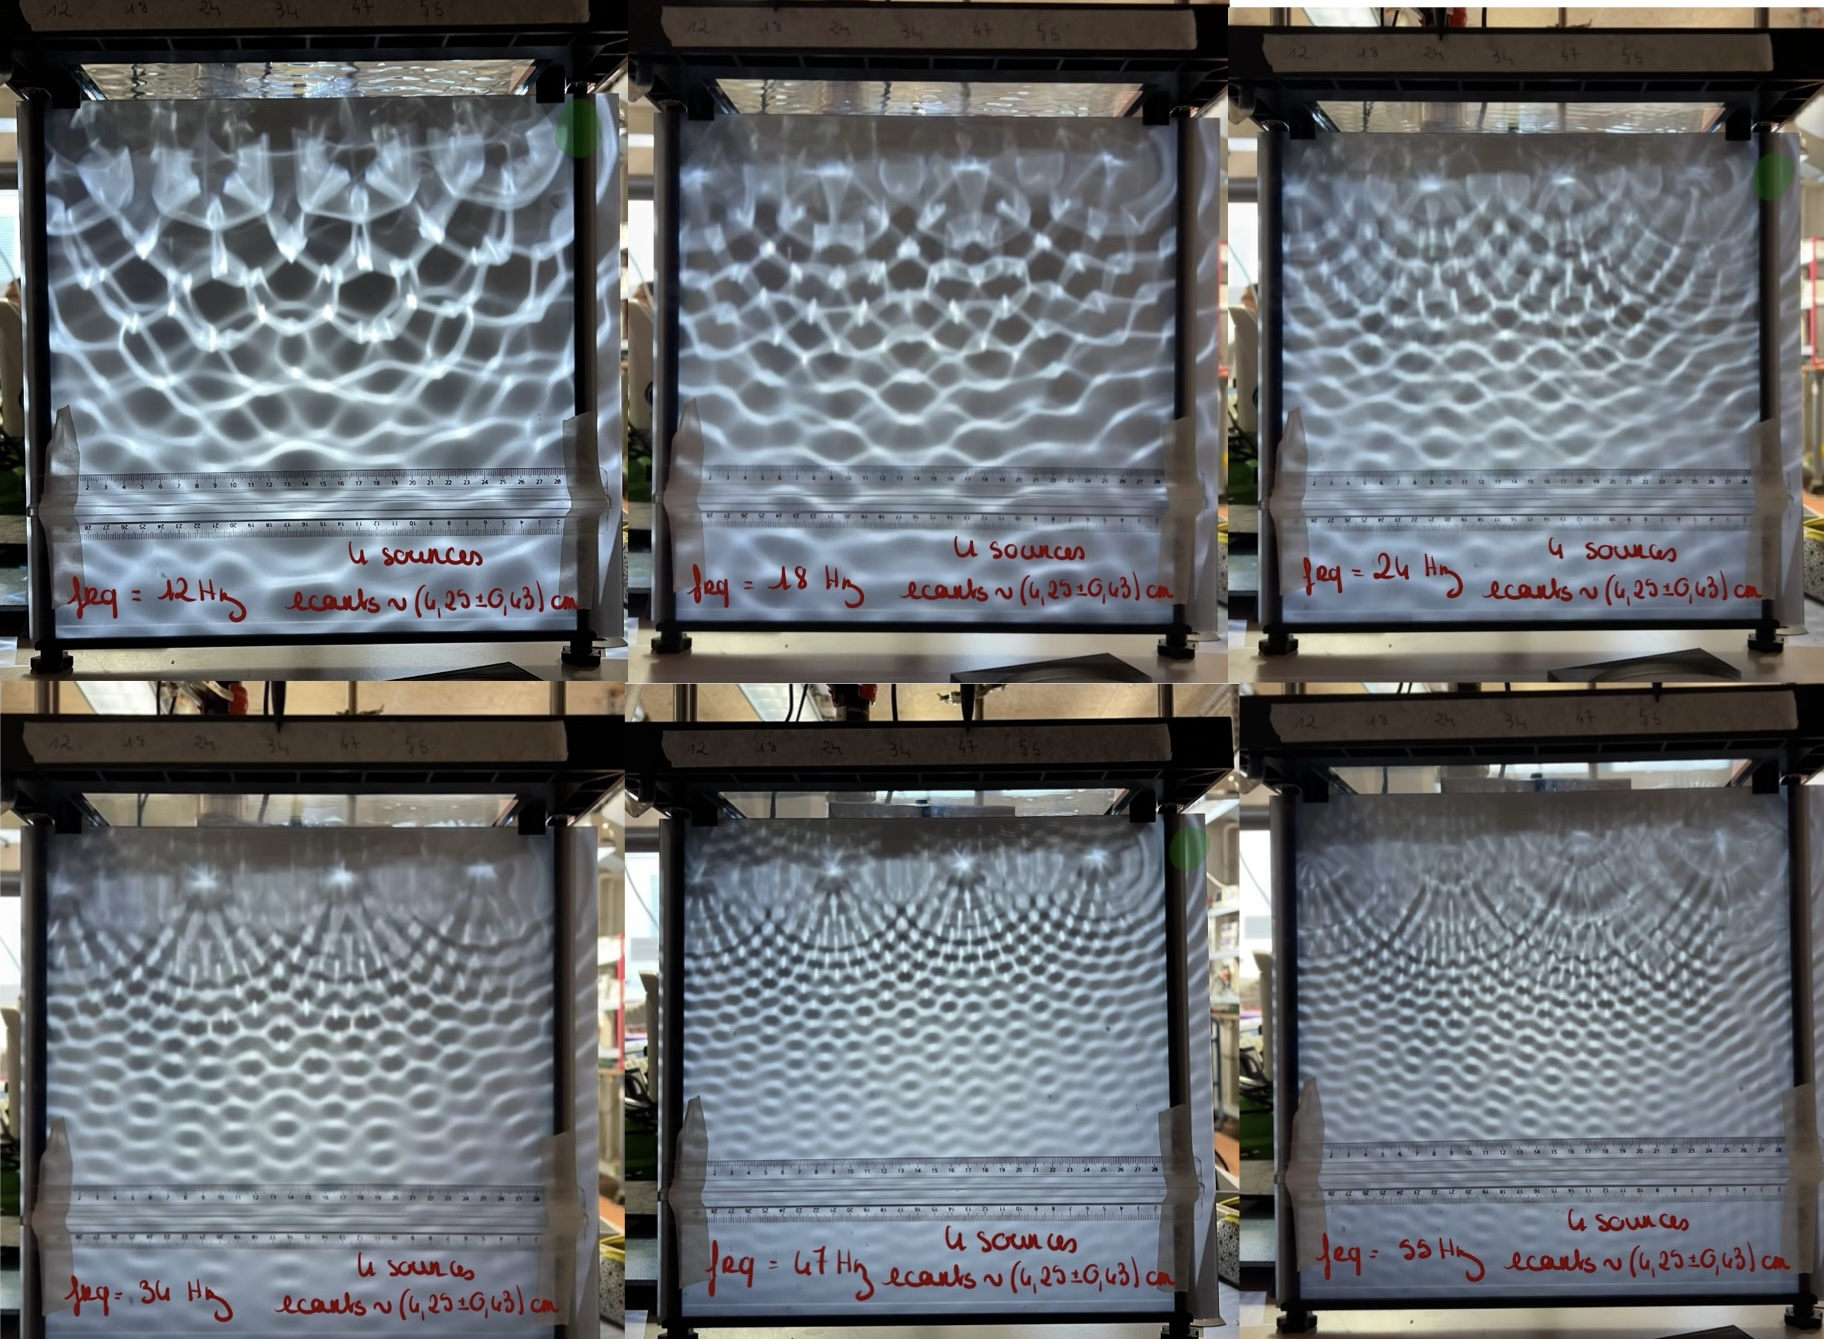
\includegraphics[scale=0.15]{S4.jpg}
    \caption{Photos avec 3 sources d'onde espacées de 4,25 cm}
    \label{fig:enter-label}
\end{figure}


\subsection{Interprétation des résultats obtenus et conclusion}

On peut remarquer que dans toutes les situations, les ondes se comportent de la même façon, elles ne sont pas déformées mais se superposent, on appelle ce phénomène le phénomène d'interférence. Si on prend l'exemple de deux sources, on remarque des comportements différents à certains endroits en particulier :

\begin{itemize}[label=\ding{239}]
    \item à certains endroits les maximas de chaque onde ou les minimas de chaque onde se croisent, les ondes se superposent et leurs amplitudes s'additionnent, on appelle cela des interférences constructives : à ces endroits, l'amplitude est maximale (en valeur absolue) : ces interférences sont toutes placées sur les lignes qu'on appelle lignes de tempête.
    \item à d'autres endroits le maximum d'une onde croise le minimum d'une autre et les ondes se superposent, et comme les deux amplitudes sont les mêmes mais l'une est négative et l'autre est positive, les amplitudes s'additionnent donc l'amplitude totale est nulle : on appelle cela des interférences destructives, et elles sont situées sur plusieurs lignes : des lignes de repos. \\
\end{itemize}

\begin{figure}[H]
\centering
\begin{minipage}{0.45\textwidth}
  \centering
  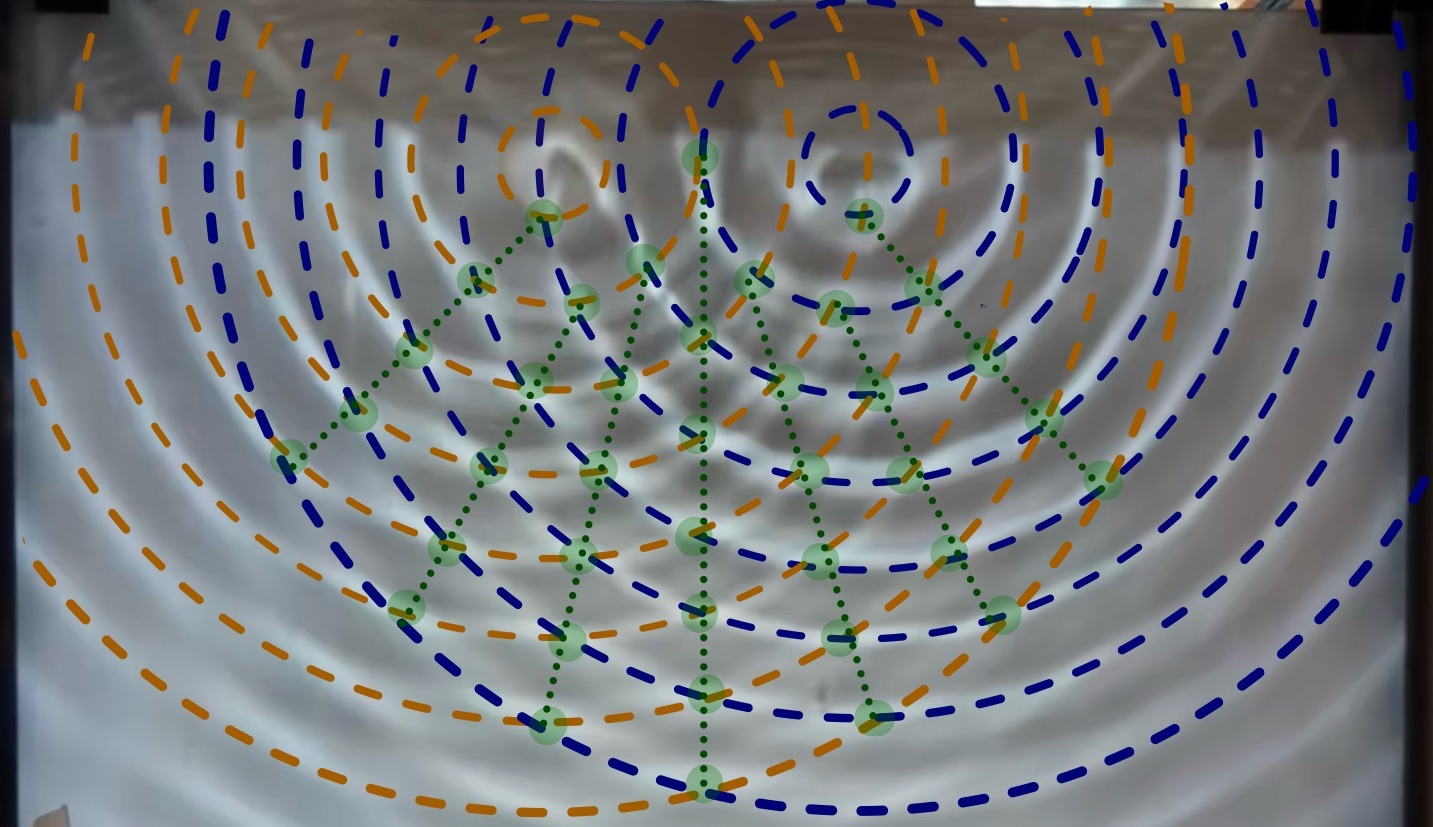
\includegraphics[scale=0.14]{tempete.JPG}
  \caption{Photo 2 sources interférences constructives}
  \label{fig:s1}
\end{minipage}\hfill
\begin{minipage}{0.45\textwidth}
  \centering
  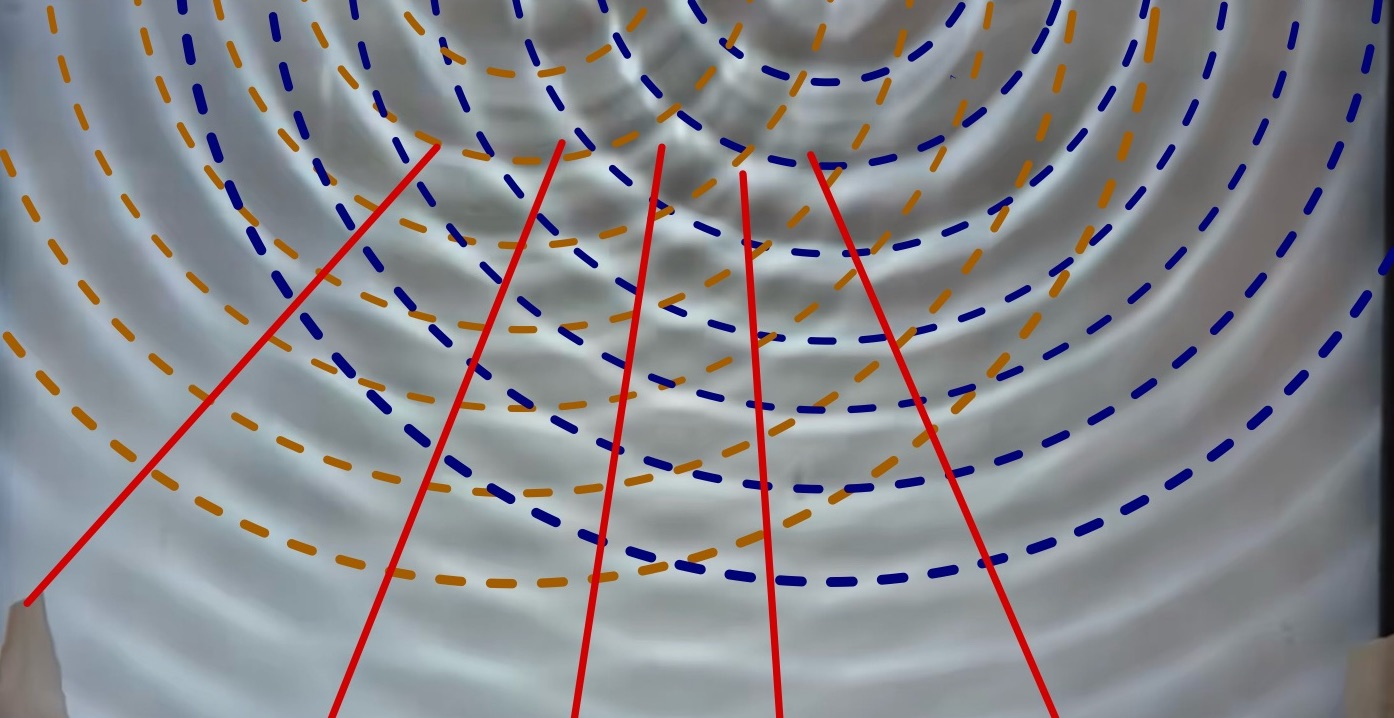
\includegraphics[scale=0.14]{repos.JPG}
  \caption{Photo 2 sources interférences destructives}
  \label{fig:s2}
\end{minipage}
\end{figure}

On peut faire d'autres observations plus précises avec la différence de marche : la différence de marche est la différence des chemins parcourus par ces deux ondes. On aura donc la différence de marche au point $X$ qui est donnée par : $\delta_X = \lvert S_1 - X \rvert - \lvert S_2 - X \rvert $, avec $S_1$ la première source et $S_2$ la deuxième source. Pour une même ligne tempête (ou de repos), on regarde la différence de marche à différents points de cette ligne : 
\newline

\begin{minipage}{0.6\textwidth}
  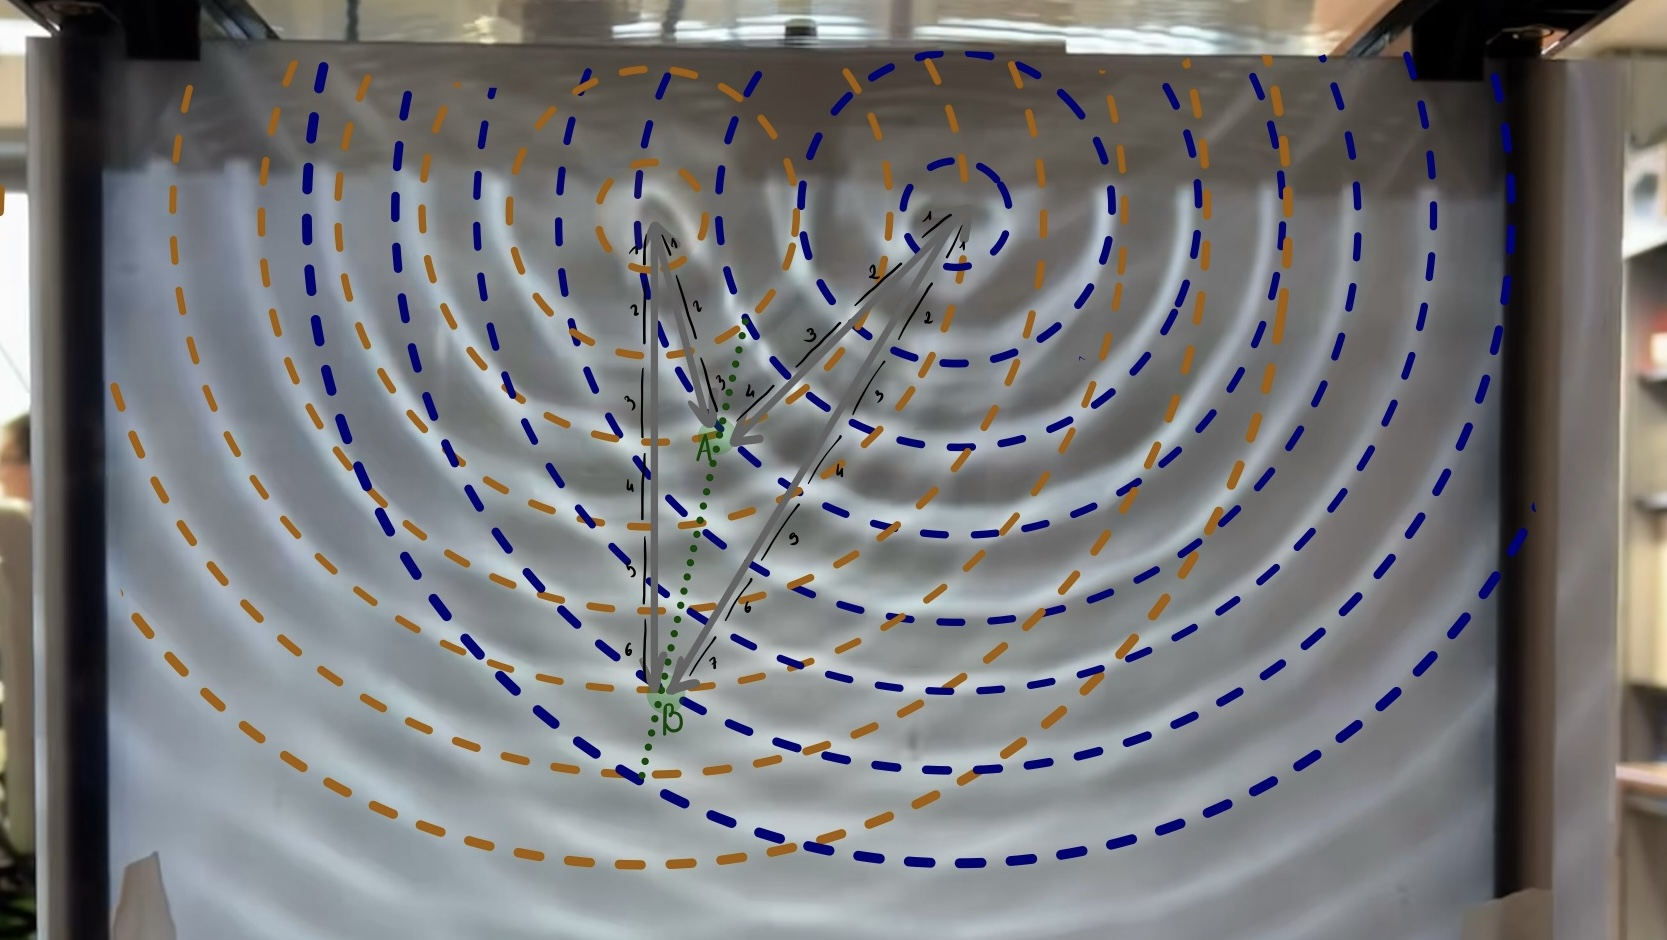
\includegraphics[scale=0.16]{calcul_tempête.jpg}
\end{minipage}
\hfill
\begin{minipage}{0.4\textwidth}
  Sur une ligne de tempête, on a :
\begin{itemize}
    \item au point A : $\delta_A = 3 \lambda - 4\lambda = -\lambda$
    \item au point B : $\delta_B = 6 \lambda - 7\lambda = -\lambda$
\end{itemize}
\end{minipage}
\newline

$\rightarrow$ interférences constructives : on trouve une différence de marche qui est un multiple de la longueur d'onde : $\delta = k \lambda$, avec $k \in \mathbb{Z}$ ; en particulier, pour chaque point d'une ligne de tempête donnée, on trouve la même différence de marche.
\newline


\begin{minipage}{0.6\textwidth}
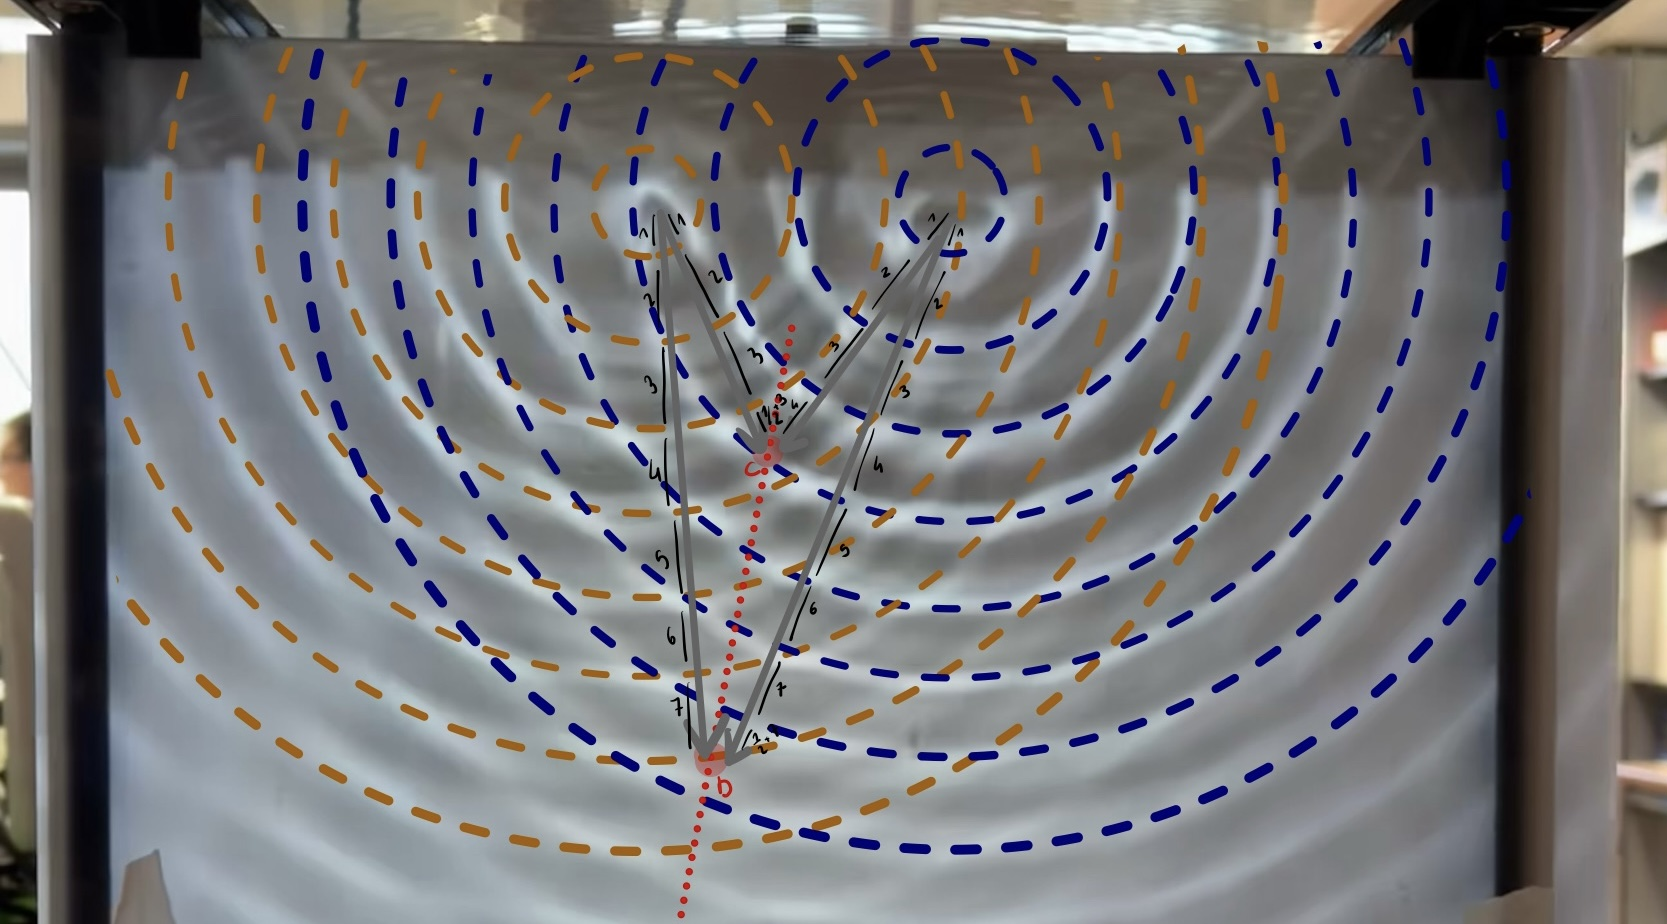
\includegraphics[scale=0.16]{calcul_repos.jpg}
\end{minipage}
\hfill
\begin{minipage}{0.4\textwidth}
  Sur une ligne de repos, on a :
\begin{itemize}
    \item au point C : $\delta_C = (3+\frac{1}{2}) \lambda - 4\lambda = -\frac{1}{2}\lambda$
    \item au point D : $\delta_D = 7 \lambda - (7+\frac{1}{2})\lambda = -\frac{1}{2}\lambda$
\end{itemize}
\end{minipage}
\newline

$\rightarrow$ interférences destructives : on trouve cette fois-ci une différence de marche qui est un multiple d'une longueur d'onde et demi c'est-à-dire $\delta = ( k + \frac{1}{2})\lambda$, avec $k \in \mathbb{Z}$ ; et dans ce cas on trouve que pour chaque point d'une ligne de repos donnée, on trouve la même différence de marche.
\newline

Pour conclure, on a donc vu qu'en présence de plusieurs sources, les ondes ne sont pas déformées, mais elles se superposent, en faisant apparaître des interférences constructives, où on distingue des lignes de tempête, et des inferférences destructives, où on distingue des lignes de repos.


\section{Diffraction}

\subsection{But et procédure}
On regarde le comportement d'une onde lorsqu'elle passe par une fente.

On génère une onde plane, et on met sur son trajet une fente pour voir le comportement de l'onde à travers cette fente.
On fait varier la taille des fentes (0,49 cm et ensuite 2,11 cm), on regarde si les caractéristiques de l'onde sont conservées :
\begin{itemize}[label=\ding{229}]
    \item on trace le graphe des longueurs d'ondes en fonction des fréquences, et on le compare aux valeurs trouvées lors de la première expérience.
    \item on prend en photo et on regarde la forme du front d'onde et l'amplitude.
\end{itemize}

\subsection{Photos, mesures et graphes}

On mesure les longueurs d'ondes à différentes fréquences pour voir si la présence de la fente a une influence sur la longueur d'onde.

\begin{table}[h]
\centering
\caption{Tableau des longueurs d'ondes en mm en présence d'une fente}
\label{tab:freq}
\begin{tabular}{c|c|c|c|c|c}
Fréquences  & $12$ Hz & $18$Hz & $24$Hz & $27$Hz & $35$Hz \\
Fente de $0,49$ cm & $18,60$ mm & $12,62$ mm & $10,10$ mm & ... & ... \\
Fente de $2,11$ cm & ... & $11,69$ mm & .... & $8,37$ mm & $6,83$ mm \\
\end{tabular}
\end{table}

\begin{figure}[H]
    \centering
    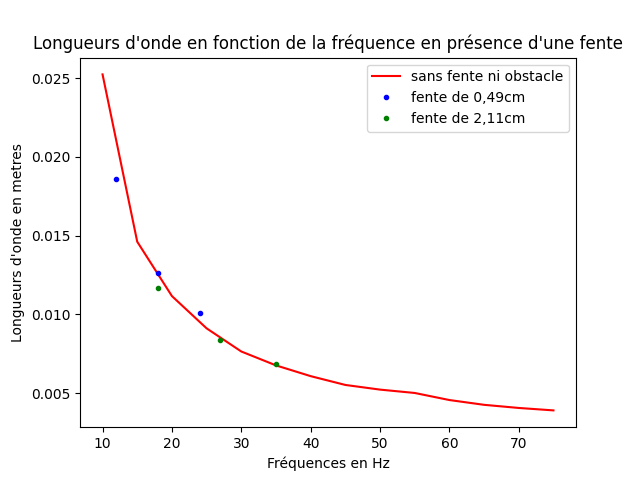
\includegraphics[scale=0.9]{fiddif.png}
    \caption{Graphe des longueurs d'onde en fonction de la fréquence en présence des fentes}
    \label{fig:enter-label}
\end{figure}

On regarde si la forme du front d'onde change en fonction de la taille de la fente. 

\begin{figure}[H]
\centering
\begin{minipage}{0.45\textwidth}
  \centering
  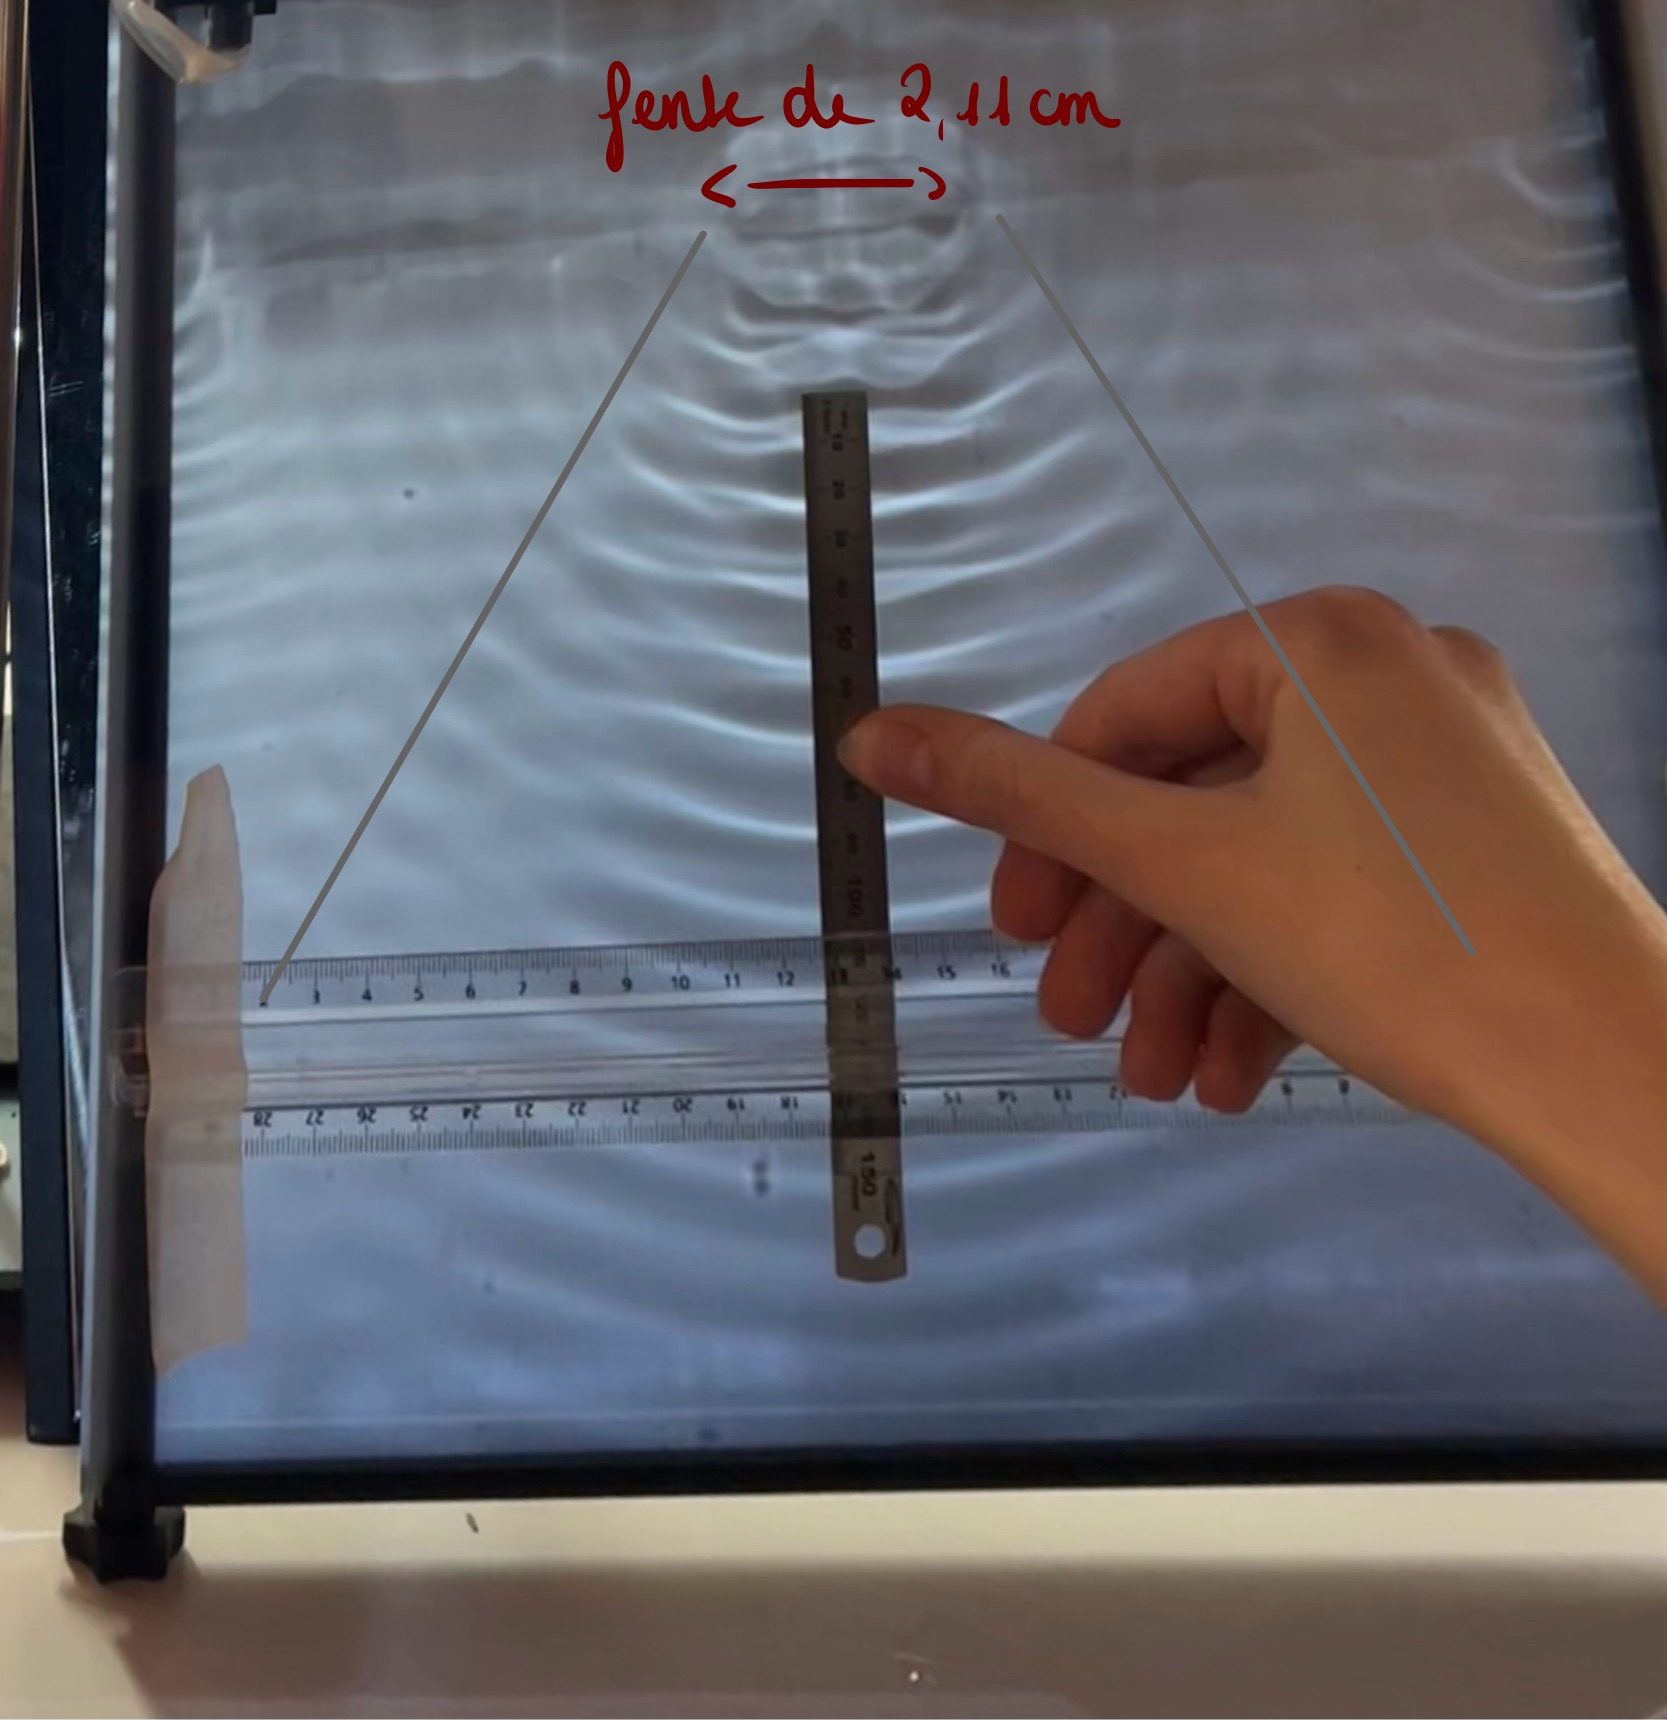
\includegraphics[scale=0.145]{petitefente.jpg}
  \caption{Photo avec une fente de 0,49 cm}
  \label{fig:s1}
\end{minipage}\hfill
\begin{minipage}{0.45\textwidth}
  \centering
  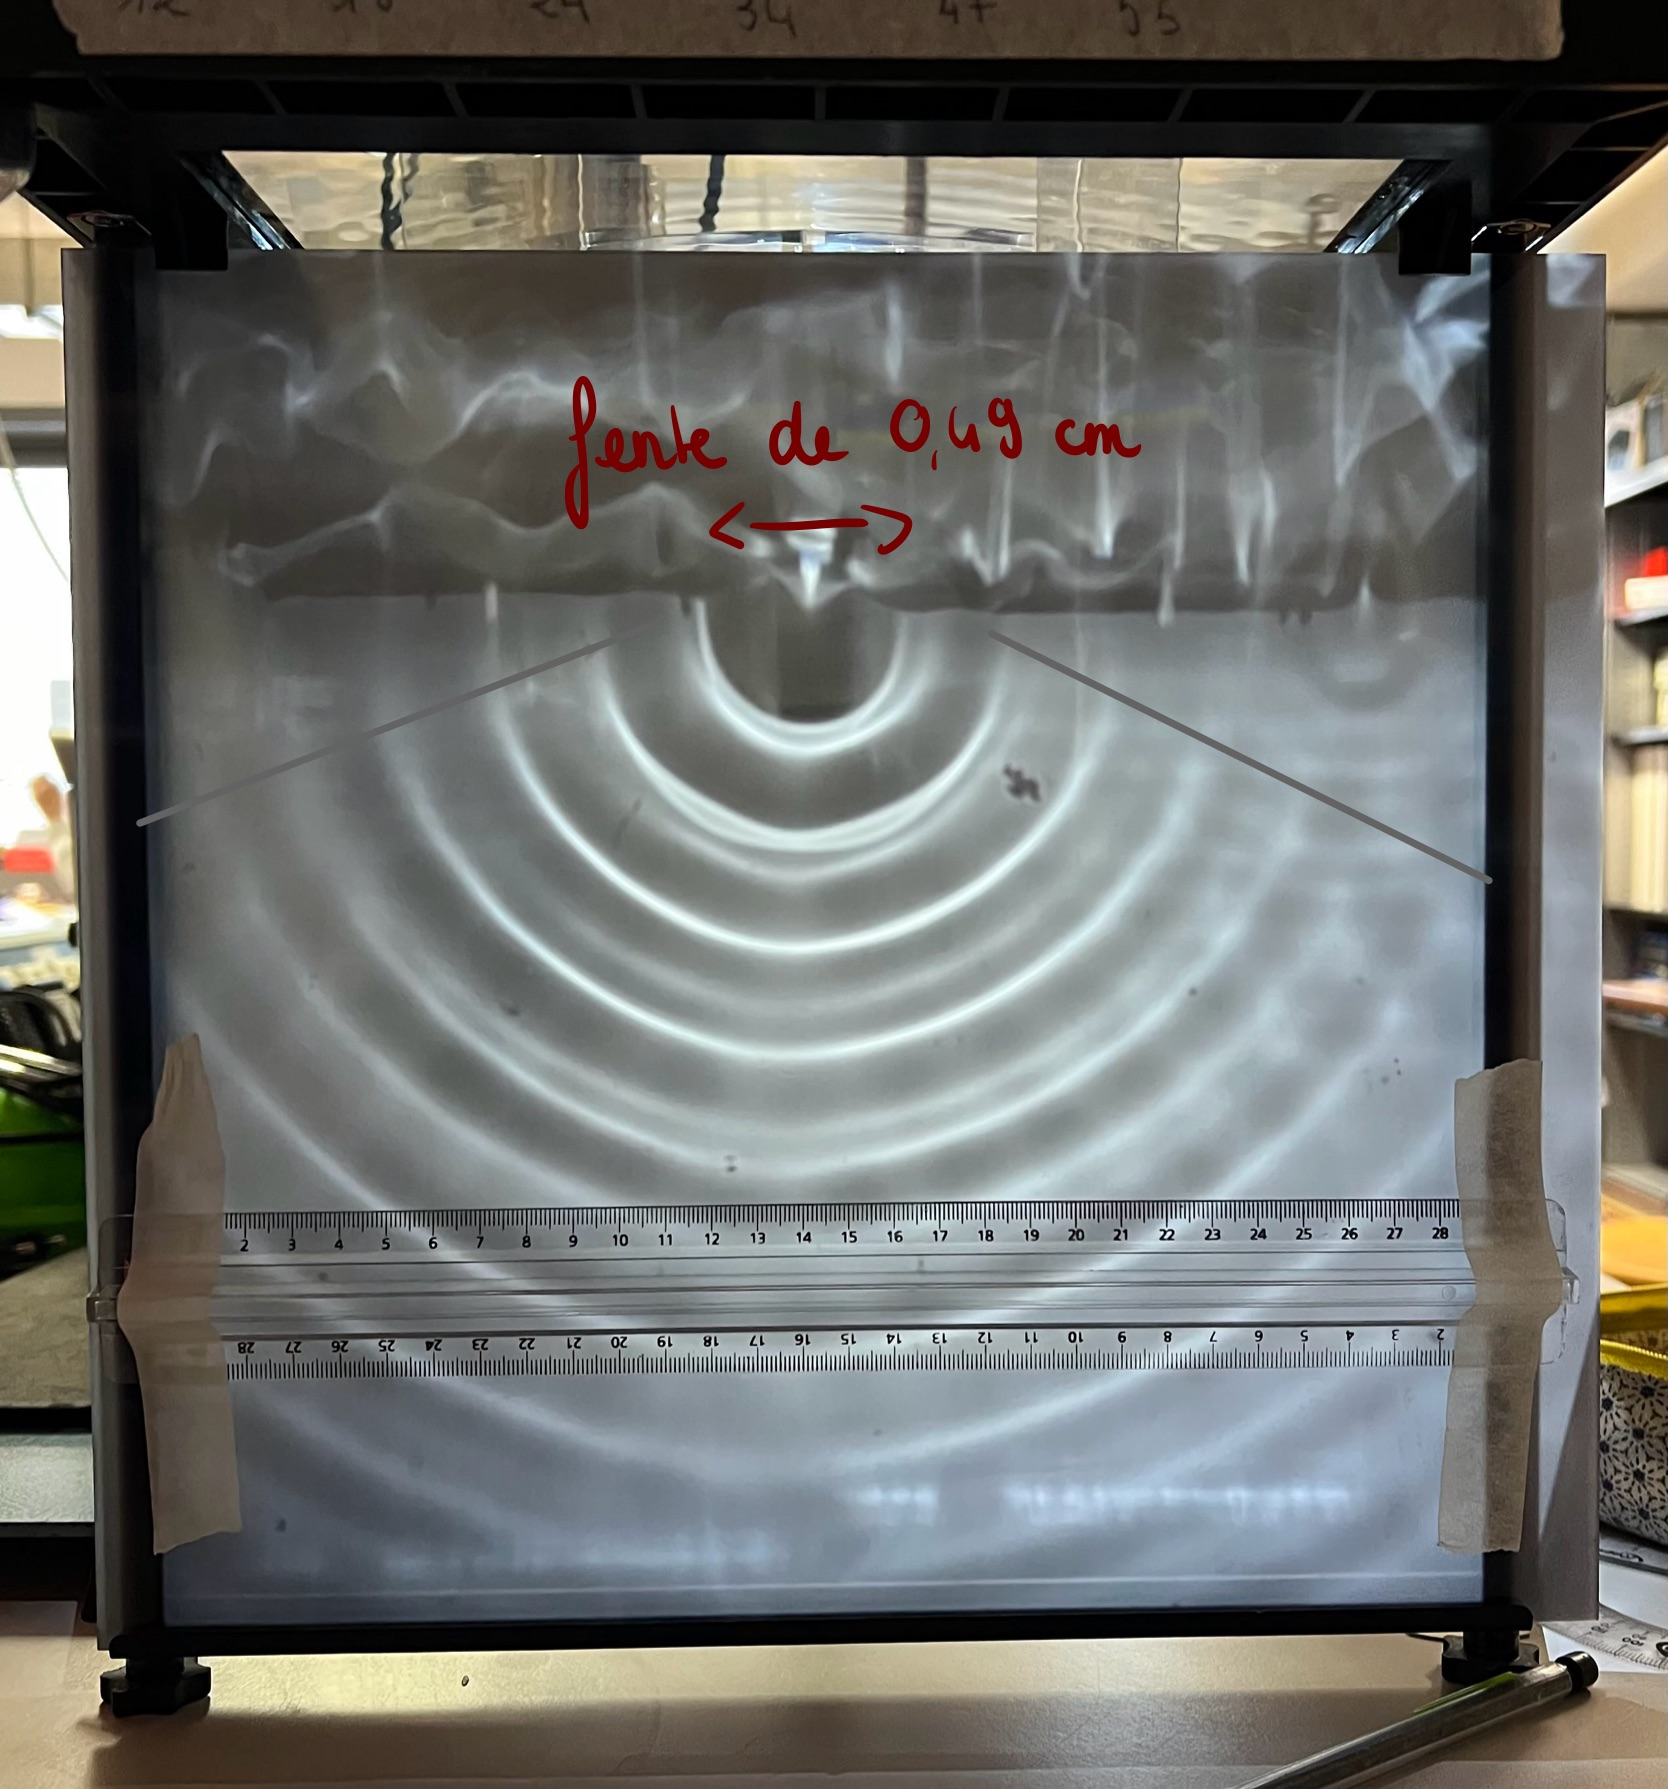
\includegraphics[scale=0.14]{grandefente.jpg}
  \caption{Photo avec une fente de 2,11 cm}
  \label{fig:s2}
\end{minipage}
\end{figure}

\subsection{Interprétation des résultats obtenus et conclusion} 
\begin{itemize}[label = \ding{217}]
    \item On a dans un premier temps vu que les fréquences sont conservées lorsque les ondes passent par une ou plusieurs fentes.
    \item On voit aussi que l'amplitude semble conservée.
    \item On peut observer des zones sombres et lumineuses de taille variable à la surface du liquide après le passage de l'onde dans la fente. On en déduit donc que des interférences destructives et constructives sont créées, comme pour l'expérience précédente.
    \item On peut néanmoins dire que le forme du front d'onde n'est pas conservée car lorsque qu'une onde passe par une fente, son front d'onde  devient alors plus courbé et elle ressemble à une onde circulaire. On voit néanmoins que plus la fente est grande, moins la forme d'onde est courbée après le passage par la fente.
\end{itemize}

\chapter{Conclusion et ouverture}

\section{Conclusion}
Pour conclure, on a observé des ondes sans dissipation dont la longueur d’onde pouvait varier entre 2mm (ondes capillaires) et 30mm (ondes de
gravité). On a aussi étudié leur relation de dispersion qui n’était pas linéaire (donc l’eau est bien un milieu dispersif). Par ailleurs on
a pu étudier comment les phénomènes d’interférence et de diffraction se manifestent sur une onde mécanique.


\section{Suggestions d'expériences}
Avec davantage de temps et de matériel, on aurait pu faire plus d'expériences :
\begin{itemize}[label=\ding{79}]
    \item Essayer de générer des ondes avec des plus grandes longueurs d'ondes et amplitudes en utilisant une cuve plus profonde : on aurait pu regarder si dans ce cas là, la relation de dispersion à la surface des fluides était toujours valable, et si le graphe avait toujours eu la même forme.

    \begin{minipage}{0.6\textwidth}
    Si on se fie à la courbe théorique, avec des longueurs d'onde variant de 10 cm à 1 m, une tension de surface de $45 mN.m^{-1}$ (celle de l'eau distillée), et une hauteur d'eau de 1 mètre, le graphe attendu devrait être de cette forme.
    \newline
    
    On voit que ce graphe n'a pas la même forme que ceux trouvés lors de la première expérience, il aurait été intéressant d'effectuer cette expérience avec ces paramètres.
    \end{minipage}
    \hfill
    \begin{minipage}{0.4\textwidth}
      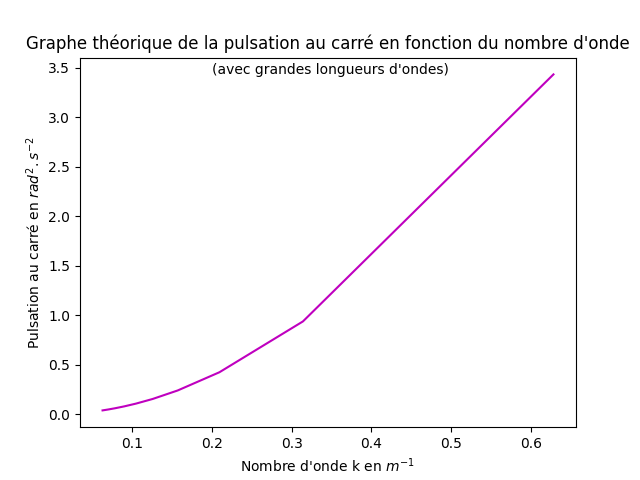
\includegraphics[scale=0.36]{graphe3.png}
    \end{minipage}

     
    \item Essayer de trouver une onde stationnaire avec un obstacle réflechissant. Nous avons essayé de faire cette expérience mais nous n'avons pas réussi car nous n'avons pas trouver de système pour éliminer les échos sur les côtés de la cuve. 

    \item Faire varier davantage la taille des fentes. On a clairement vu sur les photos qui mettaient en avant le phénomène de diffraction, que la taille de la fente avait une influence sur la forme de l'onde après être passée par la fente. Il aurait été intéressant de faire davantage de mesures en faisant varier la taille de la fente pour voir dans quel intervalle de taille de fentes on observait ce phénomène par exemple.
    
    \begin{minipage}{0.6\textwidth}
    De plus, nous avions pu remarquer en particulier sur une des photos, l'apparition d'un phénomène qui pourrait être des interférences. Nous aurions ainsi peut-être pu en déduire une relation entre la largeur de la fente, la longueur d'onde et l'angle selon lequel apparaissent les interférences. 
      \end{minipage}
    \hfill
    \begin{minipage}{0.3\textwidth}
      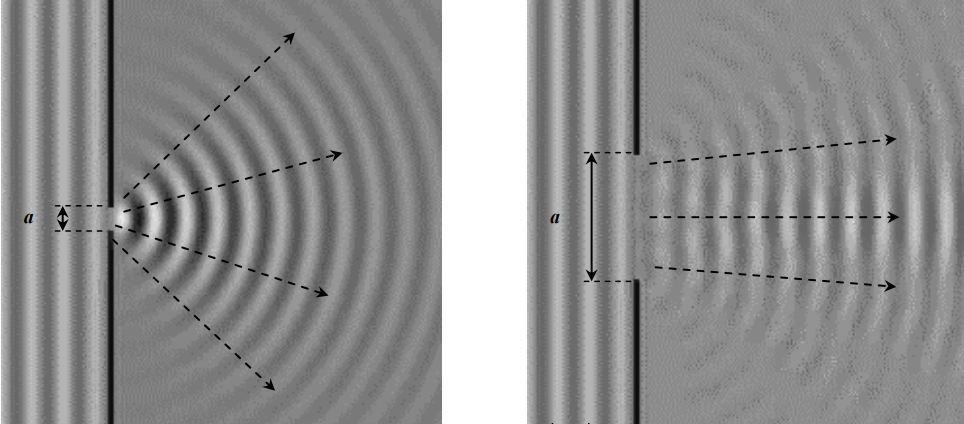
\includegraphics[scale=0.35]{conclu_diff.png}
      \caption{[5] Diffraction avec une fente plus large}
    \end{minipage}
    
    \newline
    \item Utiliser plus de fentes ainsi que des obstacles : on aurait pu utiliser des obstacles pour mettre en valeur le phénomène de diffraction dans une autre situation, ou encore utiliser plusieurs fentes pour mettre en évidence le phénomène de diffraction mais aussi peut-être d'interférence (on aura deux ondes semblables à des ondes circulaires). 

    \item Vérifier la relation de dispersion avec d'autres liquides : on aurait fait varier les masses volumiques et les tensions de surface.
    \item Utiliser une cuve plus large et plus longue pour peut-être observer de la dissipation, qui pourrait varier en fonction de la fréquence, de l'amplitude ou du liquide utilisé.
\end{itemize}
    

\begin{thebibliography}{ab}
\bibitem{image} Image extraite d'une vidéo d'expérience du site "Physique 
Ludique"
\bibitem{image} Image extraite d'une étude de document de Terminale S :"À la découverte de la diffraction et des interférences", du Lycée Jean d’Alembert / Chili.
\bibitem{image} Image extraite d'une étude de document de Terminale S :"À la découverte de la diffraction et des interférences", du Lycée Jean d’Alembert / Chili.
\bibitem{image} Image extraite d'une vidéo Youtube "TP de physique 5 : La cuve à ondes" de la chaine de l'Université de Namur.
\bibitem{image} Image extraite d'une étude sur une expérience de Terminale S: "Propriétés des ondes", du lycée Jean Mermoz

\end{thebibliography}

\end{document}